\documentclass[a4paper]{article}

\setlength{\parskip}{2mm}
\setlength{\parindent}{0pt}
\newcommand{\tab}{~ \qquad}
\usepackage{breqn}
\usepackage{ifthen}
\usepackage{amssymb}
\usepackage{multicol}
\usepackage{graphicx}
\usepackage[absolute]{textpos}
\usepackage{amsmath, amscd, amssymb, amsthm, latexsym}
% \usepackage[noload]{qtree}
%\usepackage{xspace,rotating,calligra,dsfont,ifthen}
\usepackage{xspace,rotating,dsfont,ifthen}
\usepackage[spanish,activeacute]{babel}
\usepackage[utf8]{inputenc}
\usepackage{pgfpages}
\usepackage{pgf,pgfarrows,pgfnodes,pgfautomata,pgfheaps,xspace,dsfont}
\usepackage{listings}
\usepackage{multicol}
\usepackage{todonotes}
\usepackage{url}
\usepackage{float}
\usepackage{framed,mdframed}
\usepackage{cancel}

\usepackage[strict]{changepage}


\makeatletter


\newcommand\hfrac[2]{\genfrac{}{}{0pt}{}{#1}{#2}} %\hfrac{}{} es un \frac sin la linea del medio

\newcommand\Wider[2][3em]{% \Wider[3em]{} reduce los m\'argenes
\makebox[\linewidth][c]{%
  \begin{minipage}{\dimexpr\textwidth+#1\relax}
  \raggedright#2
  \end{minipage}%
  }%
}


\@ifclassloaded{beamer}{%
  \newcommand{\tocarEspacios}{%
    \addtolength{\leftskip}{4em}%
    \addtolength{\parindent}{-3em}%
  }%
}
{%
  \usepackage[top=1cm,bottom=2cm,left=1cm,right=1cm]{geometry}%
  \usepackage{color}%
  \newcommand{\tocarEspacios}{%
    \addtolength{\leftskip}{3em}%
    \setlength{\parindent}{0em}%
  }%
}

\newcommand{\encabezadoDeProc}[4]{%
  % Ponemos la palabrita problema en tt
%  \noindent%
  {\normalfont\bfseries\ttfamily proc}%
  % Ponemos el nombre del problema
  \ %
  {\normalfont\ttfamily #2}%
  \
  % Ponemos los parametros
  (#3)%
  \ifthenelse{\equal{#4}{}}{}{%
  \ =\ %
  % Ponemos el nombre del resultado
  {\normalfont\ttfamily #1}%
  % Por ultimo, va el tipo del resultado
  \ : #4}
}

\newcommand{\encabezadoDeTipo}[2]{%
  % Ponemos la palabrita tipo en tt
  {\normalfont\bfseries\ttfamily tipo}%
  % Ponemos el nombre del tipo
  \ %
  {\normalfont\ttfamily #2}%
  \ifthenelse{\equal{#1}{}}{}{$\langle$#1$\rangle$}
}

% Primero definiciones de cosas al estilo title, author, date

\def\materia#1{\gdef\@materia{#1}}
\def\@materia{No especifi\'o la materia}
\def\lamateria{\@materia}

\def\cuatrimestre#1{\gdef\@cuatrimestre{#1}}
\def\@cuatrimestre{No especifi\'o el cuatrimestre}
\def\elcuatrimestre{\@cuatrimestre}

\def\anio#1{\gdef\@anio{#1}}
\def\@anio{No especifi\'o el anio}
\def\elanio{\@anio}

\def\fecha#1{\gdef\@fecha{#1}}
\def\@fecha{\today}
\def\lafecha{\@fecha}

\def\nombre#1{\gdef\@nombre{#1}}
\def\@nombre{No especific'o el nombre}
\def\elnombre{\@nombre}

\def\practicas#1{\gdef\@practica{#1}}
\def\@practica{No especifi\'o el n\'umero de pr\'actica}
\def\lapractica{\@practica}


% Esta macro convierte el numero de cuatrimestre a palabras
\newcommand{\cuatrimestreLindo}{
  \ifthenelse{\equal{\elcuatrimestre}{1}}
  {Primer cuatrimestre}
  {\ifthenelse{\equal{\elcuatrimestre}{2}}
  {Segundo cuatrimestre}
  {Verano}}
}


\newcommand{\depto}{{UBA -- Facultad de Ciencias Exactas y Naturales --
      Departamento de Computaci\'on}}

\newcommand{\titulopractica}{
  \centerline{\depto}
  \vspace{1ex}
  \centerline{{\Large\lamateria}}
  \vspace{0.5ex}
  \centerline{\cuatrimestreLindo de \elanio}
  \vspace{2ex}
  \centerline{{\huge Pr\'actica \lapractica -- \elnombre}}
  \vspace{5ex}
  \arreglarincisos
  \newcounter{ejercicio}
  \newenvironment{ejercicio}{\stepcounter{ejercicio}\textbf{Ejercicio
      \theejercicio}%
    \renewcommand\@currentlabel{\theejercicio}%
  }{\vspace{0.2cm}}
}


\newcommand{\titulotp}{
  \centerline{\depto}
  \vspace{1ex}
  \centerline{{\Large\lamateria}}
  \vspace{0.5ex}
  \centerline{\cuatrimestreLindo de \elanio}
  \vspace{0.5ex}
  \centerline{\lafecha}
  \vspace{2ex}
  \centerline{{\huge\elnombre}}
  \vspace{5ex}
}


%practicas
\newcommand{\practica}[2]{%
    \title{Pr\'actica #1 \\ #2}
    \author{Algoritmos y Estructuras de Datos I}
    \date{Primer Cuatrimestre 2022}

    \maketitlepractica{#1}{#2}
}

\newcommand \maketitlepractica[2] {%
\begin{center}
\begin{tabular}{r cr}
 \begin{tabular}{c}
{\large\bf\textsf{\ Algoritmos y Estructuras de Datos I\ }}\\
Primer Cuatrimestre 2022\\
\title{\normalsize Gu\'ia Pr\'actica #1 \\ \textbf{#2}}\\
\@title
\end{tabular} &
\begin{tabular}{@{} p{1.6cm} @{}}
\includegraphics[width=1.6cm]{logodpt.jpg}
\end{tabular} &
\begin{tabular}{l @{}}
 \emph{Departamento de Computaci\'on} \\
 \emph{Facultad de Ciencias Exactas y Naturales} \\
 \emph{Universidad de Buenos Aires} \\
\end{tabular}
\end{tabular}
\end{center}

\bigskip
}


% Símbolos varios

\newcommand{\nat}{\ensuremath{\mathds{N}}}
\newcommand{\ent}{\ensuremath{\mathds{Z}}}
\newcommand{\float}{\ensuremath{\mathds{R}}}
\newcommand{\bool}{\ensuremath{\mathsf{Bool}}}
\newcommand{\True}{\ensuremath{\mathrm{true}}}
\newcommand{\False}{\ensuremath{\mathrm{false}}}
\newcommand{\Then}{\ensuremath{\rightarrow}}
\newcommand{\Iff}{\ensuremath{\leftrightarrow}}
\newcommand{\implica}{\ensuremath{\longrightarrow}}
\newcommand{\IfThenElse}[3]{\ensuremath{\mathsf{if}\ #1\ \mathsf{then}\ #2\ \mathsf{else}\ #3\ \mathsf{fi}}}
\newcommand{\In}{\textsf{in }}
\newcommand{\Out}{\textsf{out }}
\newcommand{\Inout}{\textsf{inout }}
\newcommand{\yLuego}{\hspace{6pt} \land _L \hspace{6pt}}
\newcommand{\oLuego}{\hspace{6pt} \lor _L \hspace{6pt}}
\newcommand{\implicaLuego}{\implica _L }
\newcommand{\cuantificador}[5]{%
	\ensuremath{(#2 #3: #4)\ (%
		\ifthenelse{\equal{#1}{unalinea}}{
			#5
		}{
			$ % exiting math mode
			\begin{adjustwidth}{+2em}{}
			$#5$%
			\end{adjustwidth}%
			$ % entering math mode
		}
	)}
}

\newcommand{\existe}[4][]{%
	\cuantificador{#1}{\exists}{#2}{#3}{#4}
}
\newcommand{\paraTodo}[4][]{%
	\cuantificador{#1}{\forall}{#2}{#3}{#4}
}

% Símbolo para marcar los ejercicios importantes (estrellita)
\newcommand\importante{\raisebox{0.5pt}{\ensuremath{\bigstar}}}


\newcommand{\rango}[2]{[#1\twodots#2]}
\newcommand{\comp}[2]{[\,#1\,|\,#2\,]}

\newcommand{\rangoac}[2]{(#1\twodots#2]}
\newcommand{\rangoca}[2]{[#1\twodots#2)}
\newcommand{\rangoaa}[2]{(#1\twodots#2)}

%ejercicios
\newtheorem{exercise}{Ejercicio}
\newenvironment{ejercicio}[1][]{\begin{exercise}#1\rm}{\end{exercise} \vspace{0.2cm}}
\newenvironment{items}{\begin{enumerate}[a)]}{\end{enumerate}}
\newenvironment{subitems}{\begin{enumerate}[i)]}{\end{enumerate}}
\newcommand{\sugerencia}[1]{\noindent \textbf{Sugerencia:} #1}

\lstnewenvironment{code}{
    \lstset{% general command to set parameter(s)
        language=C++, basicstyle=\small\ttfamily, keywordstyle=\slshape,
        emph=[1]{tipo,usa}, emphstyle={[1]\sffamily\bfseries},
        morekeywords={tint,forn,forsn},
        basewidth={0.47em,0.40em},
        columns=fixed, fontadjust, resetmargins, xrightmargin=5pt, xleftmargin=15pt,
        flexiblecolumns=false, tabsize=2, breaklines, breakatwhitespace=false, extendedchars=true,
        numbers=left, numberstyle=\tiny, stepnumber=1, numbersep=9pt,
        frame=l, framesep=3pt,
    }
   \csname lst@SetFirstLabel\endcsname}
  {\csname lst@SaveFirstLabel\endcsname}


%tipos basicos
\newcommand{\rea}{\ensuremath{\mathsf{Float}}}
\newcommand{\cha}{\ensuremath{\mathsf{Char}}}
\newcommand{\str}{\ensuremath{\mathsf{String}}}

\newcommand{\mcd}{\mathrm{mcd}}
\newcommand{\prm}[1]{\ensuremath{\mathsf{prm}(#1)}}
\newcommand{\sgd}[1]{\ensuremath{\mathsf{sgd}(#1)}}

\newcommand{\tuple}[2]{\ensuremath{#1 \times #2}}

%listas
\newcommand{\TLista}[1]{\ensuremath{seq \langle #1\rangle}}
\newcommand{\lvacia}{\ensuremath{[\ ]}}
\newcommand{\lv}{\ensuremath{[\ ]}}
\newcommand{\longitud}[1]{\ensuremath{|#1|}}
\newcommand{\cons}[1]{\ensuremath{\mathsf{addFirst}}(#1)}
\newcommand{\indice}[1]{\ensuremath{\mathsf{indice}}(#1)}
\newcommand{\conc}[1]{\ensuremath{\mathsf{concat}}(#1)}
\newcommand{\cab}[1]{\ensuremath{\mathsf{head}}(#1)}
\newcommand{\cola}[1]{\ensuremath{\mathsf{tail}}(#1)}
\newcommand{\sub}[1]{\ensuremath{\mathsf{subseq}}(#1)}
\newcommand{\en}[1]{\ensuremath{\mathsf{en}}(#1)}
\newcommand{\cuenta}[2]{\mathsf{cuenta}\ensuremath{(#1, #2)}}
\newcommand{\suma}[1]{\mathsf{suma}(#1)}
\newcommand{\twodots}{\ensuremath{\mathrm{..}}}
\newcommand{\masmas}{\ensuremath{++}}
\newcommand{\matriz}[1]{\TLista{\TLista{#1}}}

\newcommand{\seqchar}{\TLista{\cha}}


% Acumulador
\newcommand{\acum}[1]{\ensuremath{\mathsf{acum}}(#1)}
\newcommand{\acumselec}[3]{\ensuremath{\mathrm{acum}(#1 |  #2, #3)}}

% \selector{variable}{dominio}
\newcommand{\selector}[2]{#1~\ensuremath{\leftarrow}~#2}
\newcommand{\selec}{\ensuremath{\leftarrow}}

\newcommand{\pred}[3]{%
    {\normalfont\bfseries\ttfamily\noindent pred }%
    {\normalfont\ttfamily #1}%
    \ifthenelse{\equal{#2}{}}{}{\ (#2) }%
    \{%
    \begin{adjustwidth}{+2em}{}
      \ensuremath{#3}
    \end{adjustwidth}
    \}%
    {\normalfont\bfseries\,\par}%
}

\newenvironment{proc}[4][res]{%

  % El parametro 1 (opcional) es el nombre del resultado
  % El parametro 2 es el nombre del problema
  % El parametro 3 son los parametros
  % El parametro 4 es el tipo del resultado
  % Preambulo del ambiente problema
  % Tenemos que definir los comandos requiere, asegura, modifica y aux
  \newcommand{\pre}[2][]{%
    {\normalfont\bfseries\ttfamily Pre}%
    \ifthenelse{\equal{##1}{}}{}{\ {\normalfont\ttfamily ##1} :}\ %
    \{\ensuremath{##2}\}%
    {\normalfont\bfseries\,\par}%
  }
  \newcommand{\post}[2][]{%
    {\normalfont\bfseries\ttfamily Post}%
    \ifthenelse{\equal{##1}{}}{}{\ {\normalfont\ttfamily ##1} :}\
    \{\ensuremath{##2}\}%
    {\normalfont\bfseries\,\par}%
  }
  \renewcommand{\aux}[4]{%
    {\normalfont\bfseries\ttfamily aux\ }%
    {\normalfont\ttfamily ##1}%
    \ifthenelse{\equal{##2}{}}{}{\ (##2)}\ : ##3\, = \ensuremath{##4}%
    {\normalfont\bfseries\,;\par}%
  }
  \renewcommand{\pred}[3]{%
    {\normalfont\bfseries\ttfamily pred }%
    {\normalfont\ttfamily ##1}%
    \ifthenelse{\equal{##2}{}}{}{\ (##2) }%
    \{%
    \begin{adjustwidth}{+5em}{}
      \ensuremath{##3}
    \end{adjustwidth}
    \}%
    {\normalfont\bfseries\,\par}%
  }

  \newcommand{\res}{#1}
  \vspace{1ex}
  \noindent
  \encabezadoDeProc{#1}{#2}{#3}{#4}
  % Abrimos la llave
  \{\par%
  \tocarEspacios
}
% Ahora viene el cierre del ambiente problema
{
  % Cerramos la llave
  \noindent\}
  \vspace{1ex}
}


\newcommand{\aux}[4]{%
    {\normalfont\bfseries\ttfamily\noindent aux\ }%
    {\normalfont\ttfamily #1}%
    \ifthenelse{\equal{#2}{}}{}{\ (#2)}\ : #3\, = \ensuremath{#4}%
    {\normalfont\bfseries\,;\par}%
}


% \newcommand{\pre}[1]{\textsf{pre}\ensuremath{(#1)}}

\newcommand{\procnom}[1]{\textsf{#1}}
\newcommand{\procil}[3]{\textsf{proc #1}\ensuremath{(#2) = #3}}
\newcommand{\procilsinres}[2]{\textsf{proc #1}\ensuremath{(#2)}}
\newcommand{\preil}[2]{\textsf{Pre #1: }\ensuremath{#2}}
\newcommand{\postil}[2]{\textsf{Post #1: }\ensuremath{#2}}
\newcommand{\auxil}[2]{\textsf{fun }\ensuremath{#1 = #2}}
\newcommand{\auxilc}[4]{\textsf{fun }\ensuremath{#1( #2 ): #3 = #4}}
\newcommand{\auxnom}[1]{\textsf{fun }\ensuremath{#1}}
\newcommand{\auxpred}[3]{\textsf{pred }\ensuremath{#1( #2 ) \{ #3 \}}}

\newcommand{\comentario}[1]{\text{/*\ #1\ */}}

\newcommand{\nom}[1]{\ensuremath{\mathsf{#1}}}


% En las practicas/parciales usamos numeros arabigos para los ejercicios.
% Aca cambiamos los enumerate comunes para que usen letras y numeros
% romanos
\newcommand{\arreglarincisos}{%
  \renewcommand{\theenumi}{\alph{enumi}}
  \renewcommand{\theenumii}{\roman{enumii}}
  \renewcommand{\labelenumi}{\theenumi)}
  \renewcommand{\labelenumii}{\theenumii)}
}



%%%%%%%%%%%%%%%%%%%%%%%%%%%%%% PARCIAL %%%%%%%%%%%%%%%%%%%%%%%%
\let\@xa\expandafter
\newcommand{\tituloparcial}{\centerline{\depto -- \lamateria}
  \centerline{\elnombre -- \lafecha}%
  \setlength{\TPHorizModule}{10mm} % Fija las unidades de textpos
  \setlength{\TPVertModule}{\TPHorizModule} % Fija las unidades de
                                % textpos
  \arreglarincisos
  \newcounter{total}% Este contador va a guardar cuantos incisos hay
                    % en el parcial. Si un ejercicio no tiene incisos,
                    % cuenta como un inciso.
  \newcounter{contgrilla} % Para hacer ciclos
  \newcounter{columnainicial} % Se van a usar para los cline cuando un
  \newcounter{columnafinal}   % ejercicio tenga incisos.
  \newcommand{\primerafila}{}
  \newcommand{\segundafila}{}
  \newcommand{\rayitas}{} % Esto va a guardar los \cline de los
                          % ejercicios con incisos, asi queda mas bonito
  \newcommand{\anchodegrilla}{20} % Es para textpos
  \newcommand{\izquierda}{7} % Estos dos le dicen a textpos donde colocar
  \newcommand{\abajo}{2}     % la grilla
  \newcommand{\anchodecasilla}{0.4cm}
  \setcounter{columnainicial}{1}
  \setcounter{total}{0}
  \newcounter{ejercicio}
  \setcounter{ejercicio}{0}
  \renewenvironment{ejercicio}[1]
  {%
    \stepcounter{ejercicio}\textbf{\noindent Ejercicio \theejercicio. [##1
      puntos]}% Formato
    \renewcommand\@currentlabel{\theejercicio}% Esto es para las
                                % referencias
    \newcommand{\invariante}[2]{%
      {\normalfont\bfseries\ttfamily invariante}%
      \ ####1\hspace{1em}####2%
    }%
    \newcommand{\Proc}[5][result]{
      \encabezadoDeProc{####1}{####2}{####3}{####4}\hspace{1em}####5}%
  }% Aca se termina el principio del ejercicio
  {% Ahora viene el final
    % Esto suma la cantidad de incisos o 1 si no hubo ninguno
    \ifthenelse{\equal{\value{enumi}}{0}}
    {\addtocounter{total}{1}}
    {\addtocounter{total}{\value{enumi}}}
    \ifthenelse{\equal{\value{ejercicio}}{1}}{}
    {
      \g@addto@macro\primerafila{&} % Si no estoy en el primer ej.
      \g@addto@macro\segundafila{&}
    }
    \ifthenelse{\equal{\value{enumi}}{0}}
    {% No tiene incisos
      \g@addto@macro\primerafila{\multicolumn{1}{|c|}}
      \bgroup% avoid overwriting somebody else's value of \tmp@a
      \protected@edef\tmp@a{\theejercicio}% expand as far as we can
      \@xa\g@addto@macro\@xa\primerafila\@xa{\tmp@a}%
      \egroup% restore old value of \tmp@a, effect of \g@addto.. is

      \stepcounter{columnainicial}
    }
    {% Tiene incisos
      % Primero ponemos el encabezado
      \g@addto@macro\primerafila{\multicolumn}% Ahora el numero de items
      \bgroup% avoid overwriting somebody else's value of \tmp@a
      \protected@edef\tmp@a{\arabic{enumi}}% expand as far as we can
      \@xa\g@addto@macro\@xa\primerafila\@xa{\tmp@a}%
      \egroup% restore old value of \tmp@a, effect of \g@addto.. is
      % global
      % Ahora el formato
      \g@addto@macro\primerafila{{|c|}}%
      % Ahora el numero de ejercicio
      \bgroup% avoid overwriting somebody else's value of \tmp@a
      \protected@edef\tmp@a{\theejercicio}% expand as far as we can
      \@xa\g@addto@macro\@xa\primerafila\@xa{\tmp@a}%
      \egroup% restore old value of \tmp@a, effect of \g@addto.. is
      % global
      % Ahora armamos la segunda fila
      \g@addto@macro\segundafila{\multicolumn{1}{|c|}{a}}%
      \setcounter{contgrilla}{1}
      \whiledo{\value{contgrilla}<\value{enumi}}
      {%
        \stepcounter{contgrilla}
        \g@addto@macro\segundafila{&\multicolumn{1}{|c|}}
        \bgroup% avoid overwriting somebody else's value of \tmp@a
        \protected@edef\tmp@a{\alph{contgrilla}}% expand as far as we can
        \@xa\g@addto@macro\@xa\segundafila\@xa{\tmp@a}%
        \egroup% restore old value of \tmp@a, effect of \g@addto.. is
        % global
      }
      % Ahora armo las rayitas
      \setcounter{columnafinal}{\value{columnainicial}}
      \addtocounter{columnafinal}{-1}
      \addtocounter{columnafinal}{\value{enumi}}
      \bgroup% avoid overwriting somebody else's value of \tmp@a
      \protected@edef\tmp@a{\noexpand\cline{%
          \thecolumnainicial-\thecolumnafinal}}%
      \@xa\g@addto@macro\@xa\rayitas\@xa{\tmp@a}%
      \egroup% restore old value of \tmp@a, effect of \g@addto.. is
      \setcounter{columnainicial}{\value{columnafinal}}
      \stepcounter{columnainicial}
    }
    \setcounter{enumi}{0}%
    \vspace{0.2cm}%
  }%
  \newcommand{\tercerafila}{}
  \newcommand{\armartercerafila}{
    \setcounter{contgrilla}{1}
    \whiledo{\value{contgrilla}<\value{total}}
    {\stepcounter{contgrilla}\g@addto@macro\tercerafila{&}}
  }
  \newcommand{\grilla}{%
    \g@addto@macro\primerafila{&\textbf{TOTAL}}
    \g@addto@macro\segundafila{&}
    \g@addto@macro\tercerafila{&}
    \armartercerafila
    \ifthenelse{\equal{\value{total}}{\value{ejercicio}}}
    {% No hubo incisos
      \begin{textblock}{\anchodegrilla}(\izquierda,\abajo)
        \begin{tabular}{|*{\value{total}}{p{\anchodecasilla}|}c|}
          \hline
          \primerafila\\
          \hline
          \tercerafila\\
          \tercerafila\\
          \hline
        \end{tabular}
      \end{textblock}
    }
    {% Hubo incisos
      \begin{textblock}{\anchodegrilla}(\izquierda,\abajo)
        \begin{tabular}{|*{\value{total}}{p{\anchodecasilla}|}c|}
          \hline
          \primerafila\\
          \rayitas
          \segundafila\\
          \hline
          \tercerafila\\
          \tercerafila\\
          \hline
        \end{tabular}
      \end{textblock}
    }
  }%
  % \datosalumno
}

\newcommand{\datosalumno}{
  \vspace{0.4cm}
  \textbf{Apellidos:}

  \textbf{Nombres:}

  \textbf{LU:}

  \textbf{Correo electrónico:}

  \textbf{Nro. de carillas que adjunta:}
  \vspace{0.5cm}
}


% AMBIENTE CONSIGNAS
% Se usa en el TP para ir agregando las cosas que tienen que resolver
% los alumnos.
% Dentro del ambiente hay que usar \item para cada consigna

\newcounter{consigna}
\setcounter{consigna}{0}

\newenvironment{consignas}{%
  \newcommand{\consigna}{\stepcounter{consigna}\textbf{\theconsigna.}}%
  \renewcommand{\ejercicio}[1]{\item ##1 }
  \renewcommand{\proc}[5][result]{\item
    \encabezadoDeProc{##1}{##2}{##3}{##4}\hspace{1em}##5}%
  \newcommand{\invariante}[2]{\item%
    {\normalfont\bfseries\ttfamily invariante}%
    \ ##1\hspace{1em}##2%
  }
  \renewcommand{\aux}[4]{\item%
    {\normalfont\bfseries\ttfamily aux\ }%
    {\normalfont\ttfamily ##1}%
    \ifthenelse{\equal{##2}{}}{}{\ (##2)}\ : ##3 \hspace{1em}##4%
  }
  % Comienza la lista de consignas
  \begin{list}{\consigna}{%
      \setlength{\itemsep}{0.5em}%
      \setlength{\parsep}{0cm}%
    }
}%
{\end{list}}



% para decidir si usar && o ^
\newcommand{\y}[0]{\hspace{4pt} \ensuremath{\land} \hspace{4pt}}
\newcommand{\oo}[0]{\hspace{4pt} \ensuremath{\lor} \hspace{4pt}}

% macros de correctitud
\newcommand{\semanticComment}[2]{#1 \ensuremath{#2};}
\newcommand{\namedSemanticComment}[3]{#1 #2: \ensuremath{#3};}


\newcommand{\local}[1]{\semanticComment{local}{#1}}

\newcommand{\vale}[1]{\semanticComment{vale}{#1}}
\newcommand{\valeN}[2]{\namedSemanticComment{vale}{#1}{#2}}
\newcommand{\impl}[1]{\semanticComment{implica}{#1}}
\newcommand{\implN}[2]{\namedSemanticComment{implica}{#1}{#2}}
\newcommand{\estado}[1]{\semanticComment{estado}{#1}}

\newcommand{\invarianteCN}[2]{\namedSemanticComment{invariante}{#1}{#2}}
\newcommand{\invarianteC}[1]{\semanticComment{invariante}{#1}}
\newcommand{\varianteCN}[2]{\namedSemanticComment{variante}{#1}{#2}}
\newcommand{\varianteC}[1]{\semanticComment{variante}{#1}}

\usepackage{caratula}
\usepackage{graphicx}
\usepackage{booktabs}
\usepackage{amsmath}
\usepackage{amssymb}
\usepackage[backend=bibtex,style=ieee]{biblatex}
\addbibresource{referencias.bib}

\begin{document}

\titulo{Resolviendo la Ecuación de Onda mediante la Transformada de Fourier Acelerada}
\fecha{8 de Septiembre de 2025}
\materia{Organización del Computador II}

\integrante{Polonuer, Joaquin}{1612/21}{jtpolonuer@gmail.com}

\maketitle

\tableofcontents
\newpage

\section{Introducción}

\subsection{La Ecuación de Onda}

La ecuación de onda representa uno de los fenómenos físicos más fundamentales en la naturaleza, describiendo la propagación de
perturbaciones en medios continuos. Desde ondas sonoras y electromagnéticas hasta vibraciones mecánicas, este modelo matemático
encuentra aplicación en campos tan diversos como la acústica, la óptica, la sismología y la ingeniería estructural \cite{strauss2008partial}.

La ecuación de onda unidimensional se expresa como:
\begin{equation}
    \frac{\partial^2 u}{\partial t^2} = c^2 \frac{\partial^2 u}{\partial x^2}
\end{equation}

donde $u(x,t)$ representa el desplazamiento de la onda en el punto $x$ y tiempo $t$, y $c$ es la velocidad de propagación característica del medio. Esta ecuación en derivadas parciales de segundo orden describe fenómenos como:

\begin{itemize}
    \item Vibraciones de cuerdas tensadas
    \item Propagación de ondas sonoras en tubos
    \item Ondas electromagnéticas en líneas de transmisión
\end{itemize}

Naturalmente, su extensión a dos dimensiones espaciales es:
\begin{equation}
    \frac{\partial^2 u}{\partial t^2} = c^2 \left(\frac{\partial^2 u}{\partial x^2} + \frac{\partial^2 u}{\partial y^2}\right) = c^2 \nabla^2 u
\end{equation}

Esta formulación bidimensional modela fenómenos como:

\begin{itemize}
    \item Vibraciones de membranas (tambores, diafragmas)
    \item Ondas superficiales en líquidos
    \item Propagación de ondas sísmicas en planos
    \item Ondas electromagnéticas
\end{itemize}

\subsection{La Transformada de Fourier}

La Transformada de Fourier constituye una herramienta matemática fundamental para el análisis de fenómenos ondulatorios, permitiendo
descomponer señales complejas en sus componentes frecuenciales básicas \cite{oppenheim1999discrete}. Esta transformación resulta especialmente poderosa en el
contexto de la resolución de ecuaciones diferenciales parciales \cite{strang2007computational}.

La Transformada de Fourier continua de una función $f(x)$ se define como:
\begin{equation}
    \hat{f}(\omega) = \int_{-\infty}^{\infty} f(x) e^{-i\omega x} dx
\end{equation}

y su transformada inversa:
\begin{equation}
    f(x) = \frac{1}{2\pi} \int_{-\infty}^{\infty} \hat{f}(\omega) e^{i\omega x} d\omega
\end{equation}

\subsection{Resolución de la Ecuación de Onda mediante la Transformada de Fourier}

La aplicación de la Transformada de Fourier a la ecuación de onda permite convertir la ecuación en derivadas parciales en una ecuación diferencial ordinaria,
lo que simplifica notablemente su resolución. Para abordar la ecuación (1), se aprovechan propiedades fundamentales de la transformada de Fourier relacionadas con las derivadas:

\textbf{Propiedad 1:} La transformada de Fourier de la derivada $n$-ésima de una función es igual a la multiplicación por $(i\omega)^n$ de la transformada de la función original. En particular, para $n=1$ se obtiene el caso de la derivada simple.
\begin{equation}
    \mathcal{F}\left\{\frac{\partial^n f}{\partial x^n}\right\} = (i\omega)^n \hat{f}(\omega)
\end{equation}

\textbf{Propiedad 2:} Cuando se transforma respecto a una variable diferente a la que se deriva, la derivada parcial se convierte en una derivada ordinaria de la transformada:
\begin{equation}
    \mathcal{F}_x\left\{\frac{\partial f}{\partial t}\right\} = \frac{\partial \hat{f}}{\partial t}
\end{equation}

donde $\mathcal{F}_x$ denota la transformada de Fourier respecto a la variable $x$.

Es por estas dos propiedades que al aplicar la Transformada de Fourier espacial, obtenemos:
\begin{equation}
    \frac{\partial^2 \hat{u}}{\partial t^2} = -c^2 \omega^2 \hat{u}
\end{equation}

donde $\hat{u}(\omega, t)$ es la transformada de Fourier de $u(x,t)$ respecto a $x$.

Que es ecuación diferencial ordinaria con solución analítica conocida:
\begin{equation}
    \hat{u}(\omega, t) = A(\omega) e^{ic\omega t} + B(\omega) e^{-ic\omega t}
\end{equation}

Los coeficientes $A(\omega)$ y $B(\omega)$ se determinan a partir de las condiciones iniciales, y la solución final se obtiene
aplicando la transformada inversa.

\subsection{Transformada Discreta de Fourier}

Para implementaciones computacionales, la Transformada de Fourier continua debe discretizarse. La Transformada Discreta de Fourier (DFT) de una secuencia finita $x[n]$ de $N$ elementos se define como:
\begin{equation}
    \hat{x}[k] = \sum_{n=0}^{N-1} x[n] e^{-i2\pi kn/N}, \quad k = 0, 1, \ldots, N-1
\end{equation}

donde $\hat{x}[k]$ representa los coeficientes espectrales discretos. La transformada inversa se expresa como:
\begin{equation}
    x[n] = \frac{1}{N} \sum_{k=0}^{N-1} \hat{x}[k] e^{i2\pi kn/N}, \quad n = 0, 1, \ldots, N-1
\end{equation}

La implementación directa de la DFT requiere $O(N^2)$ operaciones complejas, lo que resulta computacionalmente prohibitivo para
secuencias largas. Esta limitación motivó el desarrollo del algoritmo Fast Fourier Transform.

\subsection{Transformada Rápida de Fourier (Cooley-Tukey)}

El algoritmo FFT, desarrollado por Cooley y Tukey en 1965 \cite{cooley1965algorithm}, reduce la complejidad computacional de $O(N^2)$ a $O(N \log N)$
mediante la estrategia de divide and conquer \cite{brigham1988fast}. Para $N = 2^m$, el algoritmo descompone la DFT en DFTs más pequeñas.

El algoritmo DIT (Decimation-in-Time) separa la secuencia de entrada en muestras pares e impares:
\begin{equation}
    \hat{x}[k] = \sum_{n \text{ par}} x[n] e^{-i2\pi kn/N} + \sum_{n \text{ impar}} x[n] e^{-i2\pi kn/N}
\end{equation}

Sustituyendo $n = 2r$ para índices pares y $n = 2r+1$ para impares:
\begin{equation}
    \hat{x}[k] = \sum_{r=0}^{N/2-1} x[2r] e^{-i2\pi kr/(N/2)} + e^{-i2\pi k/N} \sum_{r=0}^{N/2-1} x[2r+1] e^{-i2\pi kr/(N/2)}
\end{equation}

Definiendo:
\begin{align}
    \hat{x}_{\text{par}}[k]   & = \sum_{r=0}^{N/2-1} x[2r] e^{-i2\pi kr/(N/2)}   \\
    \hat{x}_{\text{impar}}[k] & = \sum_{r=0}^{N/2-1} x[2r+1] e^{-i2\pi kr/(N/2)}
\end{align}

La ecuación se simplifica a:
\begin{equation}
    \hat{x}[k] = \hat{x}_{\text{par}}[k] + W_N^k \cdot \hat{x}_{\text{impar}}[k]
\end{equation}

donde $W_N^k = e^{-i2\pi k/N}$ es el factor de giro (twiddle factor).

Aprovechando la periodicidad $\hat{x}_{\text{par}}[k + N/2] = \hat{x}_{\text{par}}[k]$ y la simetría $W_N^{k+N/2} = -W_N^k$:

\begin{align}
    \hat{x}[k]       & = \hat{x}_{\text{par}}[k] + W_N^k \cdot \hat{x}_{\text{impar}}[k] \\
    \hat{x}[k + N/2] & = \hat{x}_{\text{par}}[k] - W_N^k \cdot \hat{x}_{\text{impar}}[k]
\end{align}

Este proceso se aplica recursivamente hasta obtener DFTs de un solo elemento.

\subsubsection{Algoritmo Recursivo FFT}

El algoritmo recursivo implementa directamente la estrategia divide and conquer descrita anteriormente:

\begin{verbatim}
def fft_recursive(x):
    n = len(x)
    if n <= 1:
        return x
    
    # Dividir en pares e impares
    x_par = [x[2*i] for i in range(n//2)]
    x_impar = [x[2*i+1] for i in range(n//2)]
    
    # Aplicar FFT recursivamente
    y_par = fft_recursive(x_par)
    y_impar = fft_recursive(x_impar)
    
    # Combinar resultados
    y = [0] * n
    for k in range(n//2):
        w = exp(-2j * pi * k / n)
        y[k] = y_par[k] + w * y_impar[k]
        y[k + n//2] = y_par[k] - w * y_impar[k]
    
    return y
\end{verbatim}

Este algoritmo recursivo tiene complejidad $O(N \log N)$ pero presenta overhead significativo debido a:
\begin{itemize}
    \item Creación de múltiples listas temporales
    \item Llamadas recursivas con overhead de stack
    \item Acceso no secuencial a memoria
\end{itemize}

Por esta razón, las implementaciones prácticas utilizan versiones iterativas optimizadas que mantienen la misma complejidad algorítmica pero con mejor rendimiento en la práctica \cite{duhamel1990fast}.

\subsubsection{Algoritmo Iterativo FFT}

La versión iterativa evita el overhead de la recursión mediante el uso de bit-reversal y bucles anidados:

\begin{verbatim}
def fft_iterative(x):
    n = len(x)
    if n <= 1:
        return x
    
    # Bit-reversal permutation
    j = 0
    for i in range(1, n):
        bit = n >> 1
        while j & bit:
            j ^= bit
            bit >>= 1
        j ^= bit
        if i < j:
            x[i], x[j] = x[j], x[i]
    
    # FFT iterativa
    length = 2
    while length <= n:
        w = exp(-2j * pi / length)
        for i in range(0, n, length):
            wn = 1 + 0j
            for j in range(length // 2):
                u = x[i + j]
                v = x[i + j + length // 2] * wn
                x[i + j] = u + v
                x[i + j + length // 2] = u - v
                wn *= w
        length <<= 1
    
    return x
\end{verbatim}

Esta implementación iterativa presenta varias ventajas sobre la versión recursiva:
\begin{itemize}
    \item \textbf{Acceso secuencial a memoria}: Mejor utilización de la jerarquía de cache
    \item \textbf{Sin overhead de recursión}: Elimina el costo de las llamadas a función
    \item \textbf{Menor uso de memoria}: No requiere múltiples copias de los datos
    \item \textbf{Mejor paralelización}: Los bucles pueden ser optimizados por el compilador
\end{itemize}

El algoritmo mantiene la misma complejidad $O(N \log N)$ pero con constantes significativamente menores, lo que resulta en mejor rendimiento en la práctica.

\subsection{Transformada de Fourier Bidimensional}

Para la resolución numérica de la ecuación de onda en dos dimensiones, es necesario extender la Transformada de Fourier al caso bidimensional. La Transformada Discreta de Fourier en 2D de una matriz $x[m,n]$ de dimensiones $M \times N$ se define como:
\begin{equation}
    \hat{x}[k,l] = \sum_{m=0}^{M-1} \sum_{n=0}^{N-1} x[m,n] e^{-i2\pi (km/M + ln/N)}
\end{equation}

donde $k = 0, 1, \ldots, M-1$ y $l = 0, 1, \ldots, N-1$.

La transformada inversa se expresa como:
\begin{equation}
    x[m,n] = \frac{1}{MN} \sum_{k=0}^{M-1} \sum_{l=0}^{N-1} \hat{x}[k,l] e^{i2\pi (km/M + ln/N)}
\end{equation}

Una propiedad fundamental de la FFT bidimensional es su separabilidad, que permite descomponer el cálculo en aplicaciones consecutivas de FFT unidimensionales:
\begin{equation}
    \hat{x}[k,l] = \sum_{m=0}^{M-1} e^{-i2\pi km/M} \left[ \sum_{n=0}^{N-1} x[m,n] e^{-i2\pi ln/N} \right]
\end{equation}

Esto se puede implementar eficientemente mediante el siguiente algoritmo de dos pasos:

\begin{enumerate}
    \item \textbf{FFT por filas}: Aplicar FFT 1D a cada fila de la matriz de entrada:
          \begin{equation}
              \hat{y}[m,l] = \sum_{n=0}^{N-1} x[m,n] e^{-i2\pi ln/N}
          \end{equation}

    \item \textbf{FFT por columnas}: Aplicar FFT 1D a cada columna del resultado anterior:
          \begin{equation}
              \hat{x}[k,l] = \sum_{m=0}^{M-1} \hat{y}[m,l] e^{-i2\pi km/M}
          \end{equation}
\end{enumerate}

Esto se implementa en C de la siguiente manera:
\begin{verbatim}
static void fft2d(Complex *data, int rows, int cols, int inverse)
{

    Complex *temp = (Complex *)malloc(cols * sizeof(Complex));

    for (int i = 0; i < rows; i++)
    {
        memcpy(temp, &data[i * cols], cols * sizeof(Complex));
        fft_1d(temp, cols, inverse);
        memcpy(&data[i * cols], temp, cols * sizeof(Complex));
    }

    temp = (Complex *)realloc(temp, rows * sizeof(Complex));
    for (int j = 0; j < cols; j++)
    {
        for (int i = 0; i < rows; i++)
        {
            temp[i] = data[i * cols + j];
        }
        fft_1d(temp, rows, inverse);
        for (int i = 0; i < rows; i++)
        {
            data[i * cols + j] = temp[i];
        }
    }

    free(temp);
}
\end{verbatim}

\subsubsection{Aplicación a la Ecuación de Onda}

En el contexto de la resolución de la ecuación de onda bidimensional, la FFT 2D permite transformar el operador Laplaciano $\nabla^2$ del dominio espacial al dominio frecuencial:
\begin{equation}
    \nabla^2 u(x,y) \xrightarrow{\text{FFT 2D}} -(\omega_x^2 + \omega_y^2) \hat{u}(\omega_x, \omega_y)
\end{equation}

donde $\omega_x = 2\pi k_x/L_x$ y $\omega_y = 2\pi k_y/L_y$ son las frecuencias espaciales discretas, y $L_x$, $L_y$ son las dimensiones del dominio computacional.

Esta transformación convierte la ecuación diferencial parcial en una ecuación algebraica en el dominio frecuencial, facilitando
significativamente su resolución numérica mediante métodos espectrales.

\section{Metodología}
Se propone implementar un simulador físico que permita visualizar la evolución de una onda a traves de un campo. Para esto, se desarrollaron
las interfaces `WaveSimulation2D` y `WaveVisualizer` (ver seccion experimental). A su vez, la interfaz `WaveSimulation2D` se implemento en varios
backends distintos: Python, NumPy, C, C + ASM (Assembly), y C + AVX.

El objetivo es evaluar el rendimiento de cada implementación midiendo la variable \textit{steps per second} (pasos por segundo), que
indica cuántos pasos de simulación puede procesar cada backend en un segundo. Esta métrica es fundamental para evaluar la eficiencia
computacional de diferentes enfoques de implementación.

\subsection{Implementación Propuesta}
Con el objetivo de facilitar la experimentación, se propone utilizar un diseño comun a todos los backends. A modo de ejemplo, se muestra
la implementacion de uno de ellos:

\begin{verbatim}
class ASMWaveSimulation2D:
    def __init__(self, size=256, domain_size=10.0, wave_speed=1.0, dt=0.01):
        self.c_core = c_backend_asm
        self._sim_ptr = self.c_core.create_simulation(size, domain_size, wave_speed, dt)
    
    def add_wave_source(self, x_pos, y_pos, amplitude=1.0, frequency=3.0, width=0.5):
        self.c_core.add_wave_source(self._sim_ptr, x_pos, y_pos, amplitude, frequency, width)
    
    def step(self):
        self.c_core.step_simulation(self._sim_ptr)
    
    def get_intensity(self):
        return self.c_core.get_intensity(self._sim_ptr)
    
    def get_real_part(self):
        return self.c_core.get_real_part(self._sim_ptr)
\end{verbatim}

La clase principal está hecha en Python, porque facilita la visualización. Sin embargo, toda la lógica y el procesamiento se realiza en C y Assembler. A continuación se muestra un diagrama:

\begin{figure}[h]
    \centering
    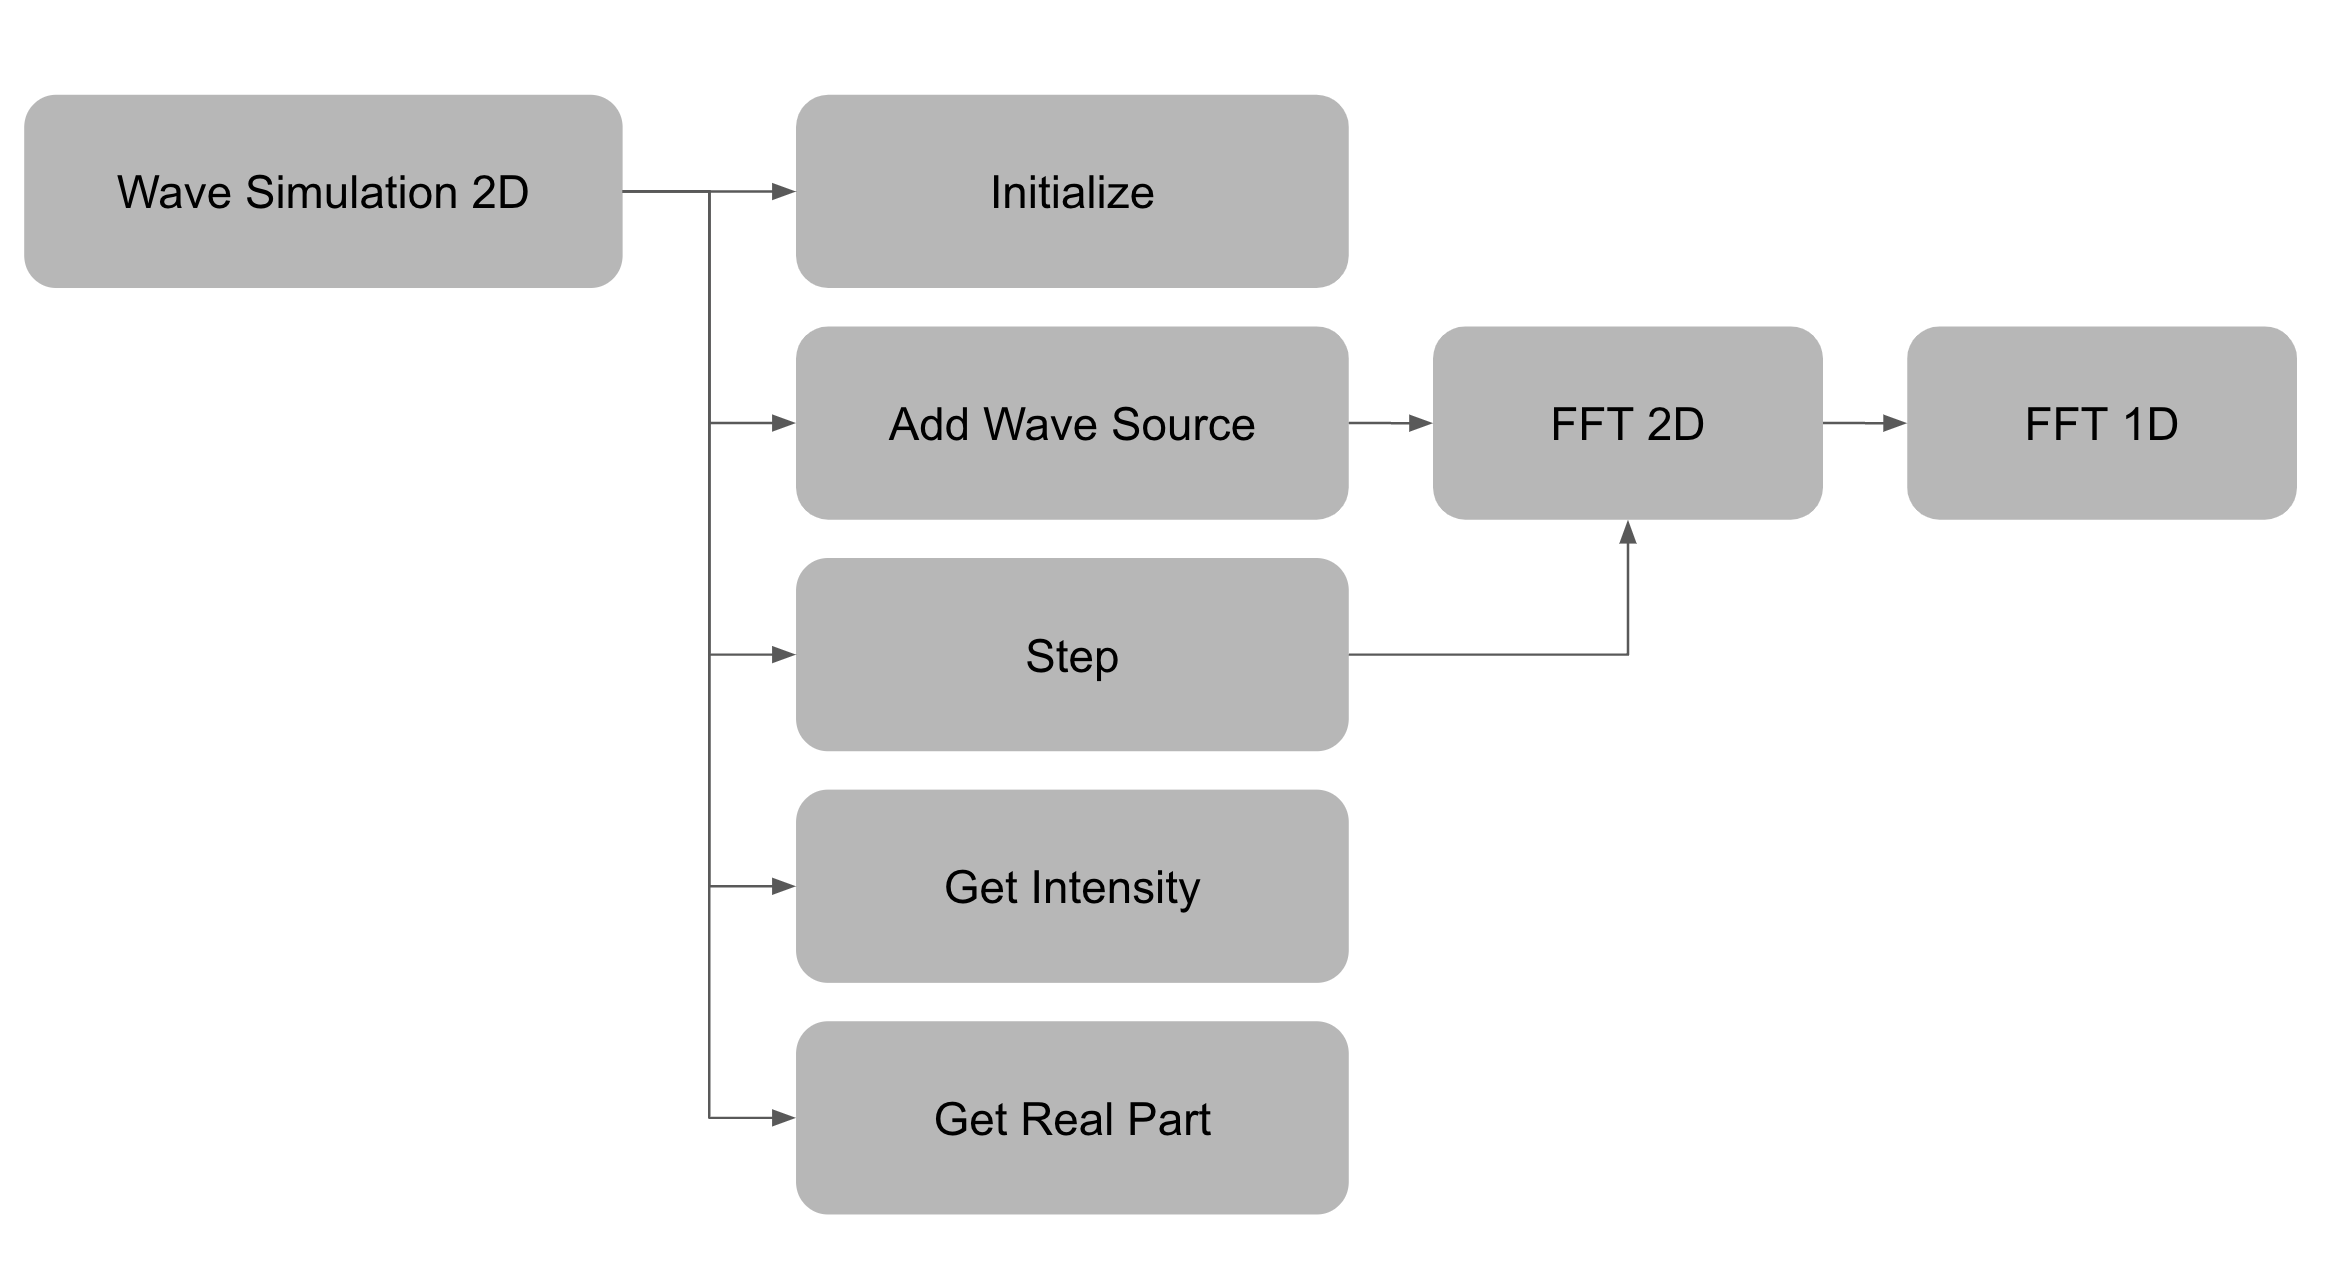
\includegraphics[width=0.7\textwidth]{extra/diagram.png}
    \caption{Diagrama de arquitectura del simulador de ondas}
    \label{fig:wave_sim_architecture}
\end{figure}

\subsubsection{Initialize} Establece el escenario matemático de la simulación: crea una grilla 2D que representa el espacio físico donde se propagarán las ondas, prepara las herramientas matemáticas (transformadas de Fourier) y define los parámetros fundamentales como la velocidad de propagación.

\subsubsection{Add Wave Source} Introduce perturbaciones localizadas en el dominio, como "tirar una piedra al agua". Genera patrones de ondas circulares que se propagan desde un punto específico, con una amplitud y frecuencia determinadas. Cada fuente crea ondas concéntricas que luego interactúan entre sí y con las ondas ya existentes.

\subsubsection{Step} Hace avanzar el tiempo de la simulación resolviendo la ecuación de ondas. Calcula cómo cada punto de la grilla cambia su altura/amplitud basándose en la física de propagación de ondas. Utiliza métodos espectrales que transforman el problema al dominio de frecuencias, donde es más eficiente calcular la evolución temporal.

\subsubsection{Get Intensity} Calcula la "intensidad" o densidad de energía en cada punto del dominio. Representa qué tan "fuerte" es la onda en cada ubicación, siempre como valores positivos. Es útil para visualizar dónde se concentra la energía de las ondas y observar patrones de interferencia constructiva.

\subsubsection{Get Real Part} Extrae la parte real del campo de ondas complejo, representando el desplazamiento físico real que veríamos. Puede ser positiva (cresta) o negativa (valle), mostrando las oscilaciones reales de la superficie. Es la representación más directa de "altura de la onda" en cada punto del espacio.

Como se ve en el diagrama, necesitamos calcular la transformada de fourier para cada paso de la simulacion. Es por esto que la
propuesta del trabajo es tratar de optimizar el algoritmo a distintos niveles y comparar sus rendimientos.

\subsection{Python y NumPy}

Para establecer un baseline de rendimiento, implementamos dos versiones en Python:

\subsubsection{Python puro} La implementación utiliza el algoritmo iterativo FFT descrito en la sección 1.5, utilizando listas de números complejos.
Esta versión sirve como referencia para entender cuánto más rápido funcionan las implementaciones en C y las librerías optimizadas como NumPy.

Esta implementación presenta limitaciones inherentes de Python:
\begin{itemize}
    \item Lentitud en operaciones numéricas
    \item Uso ineficiente de memoria, ya que las listas se almacenan de forma dispersa en memoria
\end{itemize}

\subsubsection{NumPy} Implementación optimizada que aprovecha las operaciones vectorizadas y bibliotecas optimizadas de álgebra lineal \cite{numpy2020array}. En lugar
de implementar la FFT manualmente, utilizamos directamente la función optimizada de NumPy:

\begin{verbatim}
def fft2(self, x):
    return np.fft.fft2(x)
\end{verbatim}

Como se observará en los resultados experimentales, la implementación de NumPy es extremadamente rápida y difícil de superar, aunque lograremos
un rendimiento bastante similar con nuestras implementaciones optimizadas en C.

\subsection{C}
Como se ve en \texttt{ASMWaveSimulation2D}, la clase implementada en Python es simplemente una fachada, y toda la lógica y estructuras de datos utilizadas para correr la simulación se manejan desde C. Esto funciona así en el backend de C puro, como en el de C~+~AVX y C~+~Assembler.

En el archivo \texttt{c\_backend.c} definimos dos structs fundamentales: \texttt{Complex} y \texttt{WaveSimulation}.

\begin{verbatim}
typedef struct
{
    double real;
    double imag;
} Complex;

typedef struct
{
    Complex *wave;
    Complex *wave_k;
    double *grid_coords;
    double *k_grid_coords;
    double *K;
    int size;
    double domain_size;
    double wave_speed;
    double dt;
    double dx;
} WaveSimulation;
\end{verbatim}

WaveSimulation funciona de la siguiente manera:
\begin{itemize}
    \item \textbf{grid\_coords}: Es una grilla cuadrada de un tamaño determinado (\texttt{size}). En cada posición guarda un valor $(x, y)$ que determina a qué punto del dominio equivale esa posición. En la práctica, los valores se guardan todos contiguos en memoria: $[x_0, y_0, x_1, y_1, \ldots]$.
    \item \textbf{k\_grid\_coords}: Es exactamente lo mismo pero en el dominio de las frecuencias. Recordemos que la transformada de Fourier permite resolver la ecuación diferencial fácilmente al cambiar el dominio del espacio a las frecuencias.
    \item \textbf{wave} y \textbf{wave\_k}: Funcionan en conjunto con \texttt{grid\_coords} y \texttt{k\_grid\_coords}. Tienen, para cada valor de la grilla, el valor de la función en ese punto. Básicamente, \texttt{wave[i][j] = phi(grid\_coords[i][j])}.
    \item \textbf{K}: Matriz que almacena, para cada punto en el dominio de las frecuencias, el valor de $k^2 = k_x^2 + k_y^2$, necesario para la evolución temporal de la ecuación de onda en el dominio espectral.
    \item Los demás elementos son parámetros que manejan el paso del tiempo y la velocidad de las olas. El primero no afecta la precisión de la simulación, dado que la solución utilizada es analítica. El segundo, \texttt{wave\_speed}, es un parámetro de la ecuación diferencial.
\end{itemize}

Este struct funciona gracias a tres métodos principales: \texttt{create\_wave\_simulation}, \texttt{add\_wave\_source} y \texttt{wave\_sim\_step}.

\subsubsection{create\_wave\_simulation}
\begin{itemize}
    \item Reserva memoria para la estructura \texttt{WaveSimulation} y sus arrays: \texttt{wave} y \texttt{wave\_k} de números complejos (size$^2$×Complex), \texttt{grid\_coords} y \texttt{k\_grid\_coords} (size$^2$×2×double), y \texttt{K} (size$^2$×double)
    \item Inicializa \texttt{grid\_coords} con coordenadas espaciales en formato plano [$x_0,y_0,x_1,y_1,...$] centradas en el dominio
    \item Calcula \texttt{k\_grid\_coords} usando frecuencias FFT con desplazamiento de frecuencias negativas para valores j,i > size/2
    \item Computa magnitudes \texttt{K} como $k_{mag} = \sqrt{k_x^2 + k_y^2} \times 2\pi$, evitando división por cero en k=0 con valor 1e-10
\end{itemize}

\subsubsection{add\_wave\_source}
\begin{itemize}
    \item Itera sobre todo el grid calculando la distancia radial $r^2 = (x-x_0)^2 + (y-y_0)^2$ desde la posición de la fuente
    \item Genera una envolvente gaussiana (amplitude $\times e^{-r^2/width^2}$) y fase radial (frequency $\times r$)
    \item Suma al array \texttt{wave} valores complejos envelope$\times$(cos(phase) + $i\times$sin(phase)) usando \texttt{complex\_add}
    \item Copia \texttt{wave} a \texttt{wave\_k} y aplica FFT2D directa para obtener la representación en k-space
\end{itemize}

\subsubsection{wave\_sim\_step}
\begin{itemize}
    \item Calcula evolución temporal en k-space: para cada punto obtiene $\omega$ = wave\_speed $\times$ K[idx] y phase = $-\omega \times$ dt
    \item Multiplica \texttt{wave\_k[idx]} por factor de fase complex (cos(phase) + i×sin(phase)) usando \texttt{complex\_mul}
    \item Copia \texttt{wave\_k} a \texttt{wave} y aplica FFT2D inversa para transformar de vuelta al espacio real
    \item La función preserva la ecuación de onda dispersiva aplicando el operador de evolución temporal $e^{-i\omega t}$
\end{itemize}

Estos métodos son fundamentales y, como se mencionó previamente, son la base necesaria que nos permite acelerar la simulación en todos los backends. Ya aclarado esto, la implementación de la transformada de Fourier:

\begin{verbatim}
static void fft_1d(Complex *x, int n, int inverse)
{
    assert(n > 0 && (n & (n - 1)) == 0 && "La longitud debe ser potencia de 2");

    bit_reverse(x, n);

    for (int len = 2; len <= n; len <<= 1)
    {
        double angle = 2.0 * M_PI / len * (inverse ? 1 : -1);
        Complex w = {cos(angle), sin(angle)};

        for (int i = 0; i < n; i += len)
        {
            Complex wn = {1.0, 0.0};
            for (int j = 0; j < len / 2; j++)
            {
                Complex u = x[i + j];
                Complex v = complex_mul(x[i + j + len / 2], wn);
                x[i + j] = complex_add(u, v);
                x[i + j + len / 2] = complex_sub(u, v);
                wn = complex_mul(wn, w);
            }
        }
    }

    if (inverse)
    {
        for (int i = 0; i < n; i++)
        {
            x[i].real /= n;
            x[i].imag /= n;
        }
    }
}
\end{verbatim}

\subsection{C + ASM}

La motivación de esta optimización es que necesitamos calcular la transformada todo el tiempo para volver desde el dominio de las frecuencias al dominio espacial, y esto requiere calcular la transformada en cada paso de la simulación.

La implementación en Assembler puede entenderse fácilmente haciendo un paralelismo línea por línea con la implementación en C. Sin embargo, hay algunos detalles interesantes que vale la pena mencionar.

\subsubsection{Uso de la pila x87 para operaciones matemáticas}
La arquitectura x86-64 incluye una pila de registros especializada, conocida como la \textbf{pila x87}, diseñada para operaciones matemáticas en punto flotante.
Esta pila, compuesta por ocho registros de 80 bits (st0--st7), permite realizar cálculos complejos de manera eficiente, especialmente en operaciones trigonométricas
y exponenciales, que son fundamentales para la Transformada de Fourier.

En la implementación en Assembly, la pila x87 se utiliza para calcular funciones como seno y coseno de un ángulo, aprovechando instrucciones dedicadas como
\texttt{fsin} y \texttt{fcos}. El flujo típico consiste en cargar el ángulo en la pila, calcular el seno (dejando el ángulo aún disponible en la pila), almacenar
el resultado en memoria, y luego calcular el coseno sobre el mismo ángulo. Finalmente, ambos resultados se transfieren a registros xmm para su uso vectorizado.

El siguiente fragmento ilustra este proceso, equivalente a la operación en C \texttt{Complex w = {cos(angle), sin(angle)}}:
\begin{verbatim}
.declarar_w:
fld     st0                             ; Copio el angulo devuelta en st0, st1 = angulo
fsin                                    ; st0 = sin(ang)   (ángulo sigue en st1)
fstp    qword [rsp]                     ; guardar sin en memoria
movhpd  xmm6, [rsp]                     ; xmm6 = [?, w_i]

fcos                                    ; st0 = cos(ang)
fstp    qword [rsp]                     ; guardar cos
movlpd   xmm6, [rsp]                     ; xmm6 = [w_r, w_i]
; (pila x87 vacía)
\end{verbatim}
En este código, se observa cómo la pila x87 permite calcular ambas funciones trigonométricas sin necesidad de recalcular el ángulo ni acceder repetidamente a memoria, optimizando así el rendimiento en operaciones matemáticas intensivas.


\subsubsection{Representación de números complejos}
Dado que la Transformada de Fourier trabaja con números complejos, es fundamental definir cómo vamos a manejarlos en Assembler. Como vimos en la implementación de C, la función recibe un puntero a un arreglo de complejos. Como ya vimos antes, el tipo de dato \texttt{Complex} ocupa 128 bits, o dos doubles, por lo que resulta ideal usar registros xmm para operar con ellos. En este trabajo, trabajamos con números complejos en los registros xmm de la siguiente manera:

\begin{figure}[h]
    \centering
    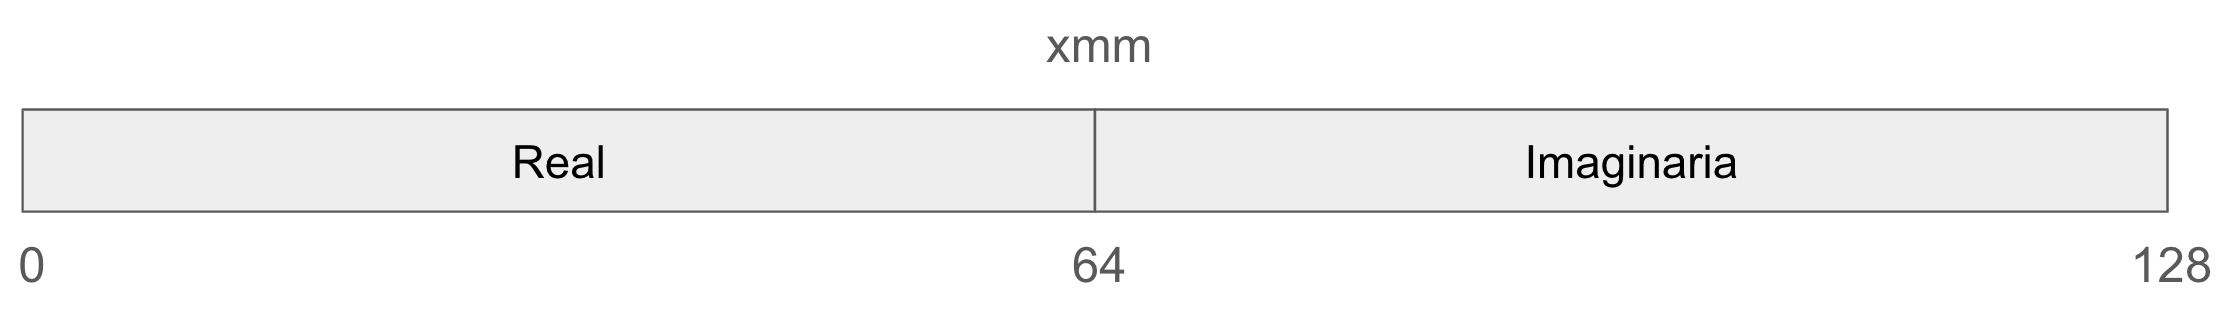
\includegraphics[width=0.5\textwidth]{extra/xmm complex.png}
    \caption{Representación de números complejos en memoria para la implementación en Assembly}
    \label{fig:asm_complex_representation}
\end{figure}
Esta representación no solo permite hacer solo una lectura de memoria por cada complejo, lo cual es razonable, sino que además permite aprovechar las instrucciones de packed double para paralelizar sumas y restas, es decir, al sumar dos números complejos, la suma de la parte real e imaginaria se realiza simultáneamente.

\begin{verbatim}
; --------------- x[i + j] = complex_add(u, v) --------------
movapd  xmm11, xmm0                     ; xmm11 = u_r, u_i
addpd   xmm11, xmm4                     ; xmm11 = u_r + v_r, u_i + v_i
movapd  [rdi],   xmm11
\end{verbatim}

Otro detalle interesante de la implementación en Assembler es la utilización de una macro para el cálculo de la multiplicación compleja, dado que la misma se utiliza más de una vez. Esto resulta conveniente porque:

\begin{itemize}
    \item Facilita la edición del código si queremos hacer optimizaciones posteriores
    \item Al añadirse al código al momento de compilar, no tiene efectos en la performance, como sí tendría utilizar una función
\end{itemize}

La macro se define de la siguiente manera:

\begin{verbatim}
; Macro para multiplicación compleja: result = a * b
; Parámetros: a, b, result
; Fórmula: (a_r + a_i*i) * (b_r + b_i*i) = (a_r*b_r - a_i*b_i) + (a_r*b_i + a_i*b_r)*i
%macro COMPLEX_MUL 3
    movapd  %3, %1                      ; t1 = a
    mulpd   %3, %2                      ; t1 = [ar*br, ai*bi]
    xorpd   %3, [rel COMPLEX_NEGHI]     ; t1 = [ar*br, -(ai*bi)]

    movapd  xmm15, %1
    shufpd  xmm15, xmm15, 1   ; xmm15 = [ai, ar]
    mulpd   xmm15, %2         ; xmm15 = [ai*br, ar*bi]

    haddpd  %3, xmm15         ; %3 = [ar*br - ai*bi, ai*br + ar*bi]
%endmacro
\end{verbatim}

Y utiliza una mascara definida en la seccion .rodata que permite negar la parte imaginaria del numero.

\subsection{C + AVX}
Como se mencionó en la sección anterior, cada número complejo ocupa 128 bits, por lo que el uso de los registros xmm, a pesar de permitir paralelizar las operaciones efectivamente, solo soporta operar sobre un elemento del arreglo a la vez. Es por esto que se propone utilizar AVX para acelerar el ciclo interno de la transformada, habitualmente llamado \textit{butterfly}.

AVX2 (Advanced Vector Extensions 2) es una extensión del conjunto de instrucciones x86-64 introducida por Intel en 2013 \cite{intel2016intrinsics}. Los registros introducidos duplican el ancho
de los registros SSE (128 bits), por lo que permiten operar sobre 4 valores double precision simultáneamente \cite{fog2016optimizing}.

\subsubsection{Representación de números complejos}

El uso de estos registros es analogo al explicado en la implementacion de C + ASM, solo que guardando dos numeros complejo por cada registro ymm:

\begin{figure}[h]
    \centering
    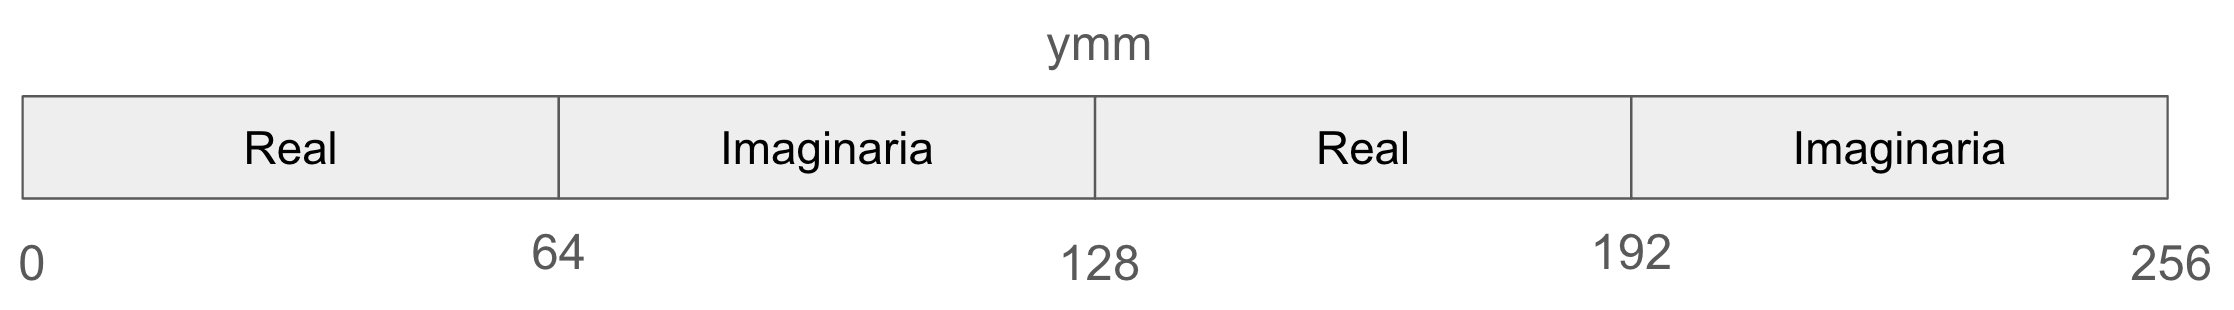
\includegraphics[width=0.7\textwidth]{extra/ymm complex.png}
    \caption{Esquema del ciclo butterfly vectorizado con AVX para la FFT}
    \label{fig:avx_butterfly}
\end{figure}

Para simplificar la implementación y aprovechar las optimizaciones realizadas por el compilador, utilizamos C para añadir estas operaciones \textit{inline}.

\subsubsection{Implementación del Ciclo Butterfly}

La implementación AVX mantiene la misma estructura algorítmica que las versiones anteriores, con la diferencia clave en el ciclo butterfly, donde se procesan
múltiples elementos simultáneamente. Las funciones que permiten esta aceleración son:
\begin{itemize}
    \item \texttt{\_mm256\_loadu\_pd}: Carga 256 bits de memoria como 4 packed doubles.
    \item \texttt{\_mm256\_setr\_pd}: Carga 4 doubles en un registro avx.
    \item \texttt{\_mm256\_add\_pd} y \texttt{\_mm256\_sub\_pd}: Similares a addpd y subpd de Assembler, suma 4 packed doubles, posición a posición.
    \item \texttt{\_mm256\_mul\_pd}: Multiplica 4 packed doubles, posición a posición.
    \item \texttt{\_mm256\_hadd\_pd} y \texttt{\_mm256\_hsub\_pd}: Realizan sumas y restas horizontales entre pares de elementos del registro.
    \item \texttt{\_mm256\_storeu\_pd}: Guarda 4 packed doubles en memoria.
\end{itemize}

Y vale la pena detenerse a considerar la implementación de \texttt{complex\_mul\_simd}, dado que utiliza operaciones interesantes:
\begin{verbatim}
// Recibe: z1 = [a1, b1, a2, b2], z2 = [c1, d1, c2, d2]
// Devuelve: [(a1*c1-b1*d1), (a1*d1+b1*c1), (a2*c2-b2*d2), (a2*d2+b2*c2)]
static inline __m256d complex_mul_simd(__m256d z1, __m256d z2)
{
    __m256d ac_bd = _mm256_mul_pd(z1, z2);               // ac_bd = [a1*c1, b1*d1, a2*c2, b2*d2]
    __m256d z2_swapped = _mm256_shuffle_pd(z2, z2, 0x5); // z2_swapped = [d1, c1, d2, c2] (intercambio real/imag)
    __m256d ad_bc = _mm256_mul_pd(z1, z2_swapped);       // ad_bc = [a1*d1, b1*c1, a2*d2, b2*c2]

    __m256d real_parts = _mm256_hsub_pd(ac_bd, ac_bd); // real_parts = [a1*c1-b1*d1, a1*c1-b1*d1, a2*c2-b2*d2, a2*c2-b2*d2]
    __m256d imag_parts = _mm256_hadd_pd(ad_bc, ad_bc); // imag_parts = [a1*d1+b1*c1, a1*d1+b1*c1, a2*d2+b2*c2, a2*d2+b2*c2]

    return _mm256_unpacklo_pd(real_parts, imag_parts); // Resultado = [a1*c1-b1*d1, a1*d1+b1*c1, a2*c2-b2*d2, a2*d2+b2*c2]
}
\end{verbatim}

\section{Experimentos}

Se realizaron experimentos para evaluar el rendimiento de cada backend implementado. Para cada backend, testeamos el correcto funcionamiento mediante una simulacion interactiva, y medimos
el rendimiento en distintos tamaños.

Los experimentos se realizaron en un sistema con las siguientes especificaciones:
\begin{itemize}
    \item \textbf{Procesador}: Intel x86-64 con soporte para AVX2
    \item \textbf{Sistema Operativo}: Linux 6.8.0-78-generic
    \item \textbf{Compilador}: GCC sin optimizaciones específicas (compilación por defecto)
    \item \textbf{Parámetros de simulación}:
          \begin{itemize}
              \item Tamaño del dominio: 8.0 unidades
              \item Velocidad de onda: 2.0 unidades/segundo
              \item Intervalo de tiempo: 0.02 segundos
              \item Pasos de simulación: 50 (para medición de rendimiento)
          \end{itemize}
\end{itemize}

Se evaluaron seis implementaciones diferentes:
\begin{enumerate}
    \item \textbf{Python}: Implementación en Python puro como baseline
    \item \textbf{NumPy}: Utilizando la biblioteca NumPy optimizada
    \item \textbf{C}: Implementación en C con optimizaciones del compilador
    \item \textbf{C + ASM}: C con rutinas críticas en Assembly x86-64
    \item \textbf{C + AVX}: Utilizando extensiones AVX para paralelización vectorial
\end{enumerate}

\subsection{Visualización Interactiva}
Obviamente, una parte fundamental del trabajo es poder visualizar interactivamente la simulación. Por ese motivo, se implementó una visualización que permite agregar ondas haciendo clic en cualquier lugar del campo.

\begin{figure}[h]
    \centering
    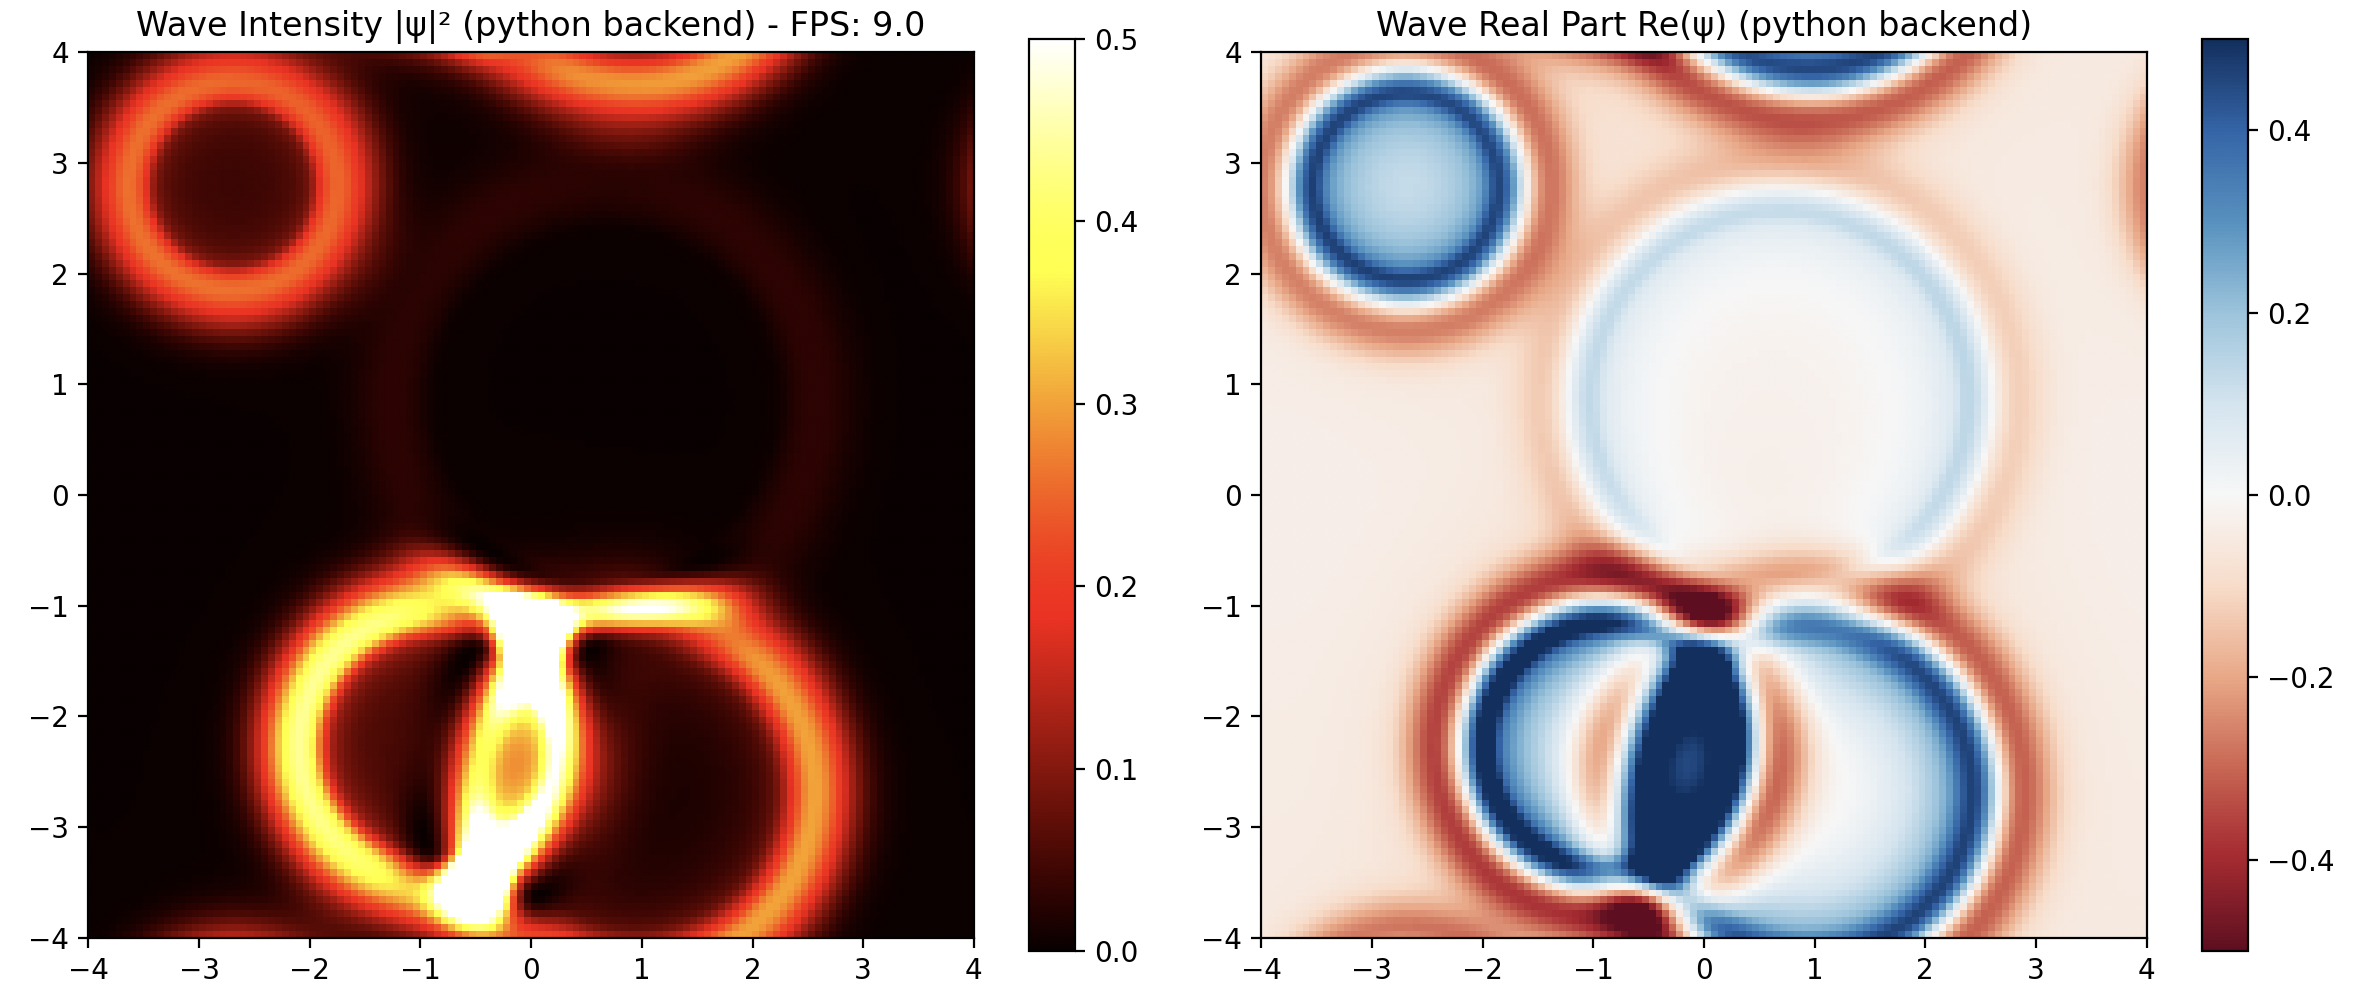
\includegraphics[width=0.8\textwidth]{extra/live_visualization.png}
    \caption{Visualización interactiva del simulador de ondas 2D}
    \label{fig:live_visualization}
\end{figure}

\subsection{Rendimiento por Tamaño de Grilla}
Una vez verificado el correcto funcionamiento de cada backend, decidimos medir más precisamente la performance. Para esto, dejamos de lado la visualización y simplemente medimos cantidad de pasos que puede computar la simulacion por segundo. Básicamente, nos importa cuánto tarda en correr la función \texttt{step} en cada uno de los backends.

Un paréntesis importante es que, a los efectos de la visualización, las implementaciones en C tienen un pequeño \textit{overhead} porque deben convertir su grilla a un numpy array y esto consume un tiempo extra. En este trabajo evitamos lidiar con eso y simplemente medimos el tiempo que tarda en correr cada paso de la simulación, porque es lo que decidimos optimizar. \\

\begin{table}[h]
    \centering
    \caption{Rendimiento de diferentes implementaciones (steps per second)}
    \label{tab:performance_results}
    \begin{tabular}{lccccccc}
        \toprule
        \textbf{Método} & \textbf{16×16}       & \textbf{32×32}       & \textbf{64×64}      & \textbf{128×128}    & \textbf{256×256}  & \textbf{512×512} & \textbf{1024×1024} \\
        \midrule
        Python          & 626,5                & 154,3                & 37,3                & 9,1                 & 2,1               & 0,5              & 0,1                \\
        ASM             & 54.928,0             & 16.541,7             & 4.321,6             & \underline{1.064,1} & \underline{245,3} & \underline{57,2} & 12,0               \\
        C               & \underline{56.649,2} & 14.737,5             & 3.341,2             & 789,0               & 178,1             & 41,6             & 9,4                \\
        C\_AVX          & \textbf{65.495,1}    & \underline{18.320,5} & \underline{4.338,2} & 1.026,6             & 230,9             & 53,7             & \underline{12,2}   \\
        Numpy           & 19.148,6             & \textbf{12.521,8}    & \textbf{5.472,7}    & \textbf{1.610,4}    & \textbf{368,8 }   & \textbf{88,5}    & \textbf{15,7}      \\
        \bottomrule
    \end{tabular}
\end{table}

\begin{figure}[H]
    \centering
    \begin{minipage}[t]{0.48\textwidth}
        \centering
        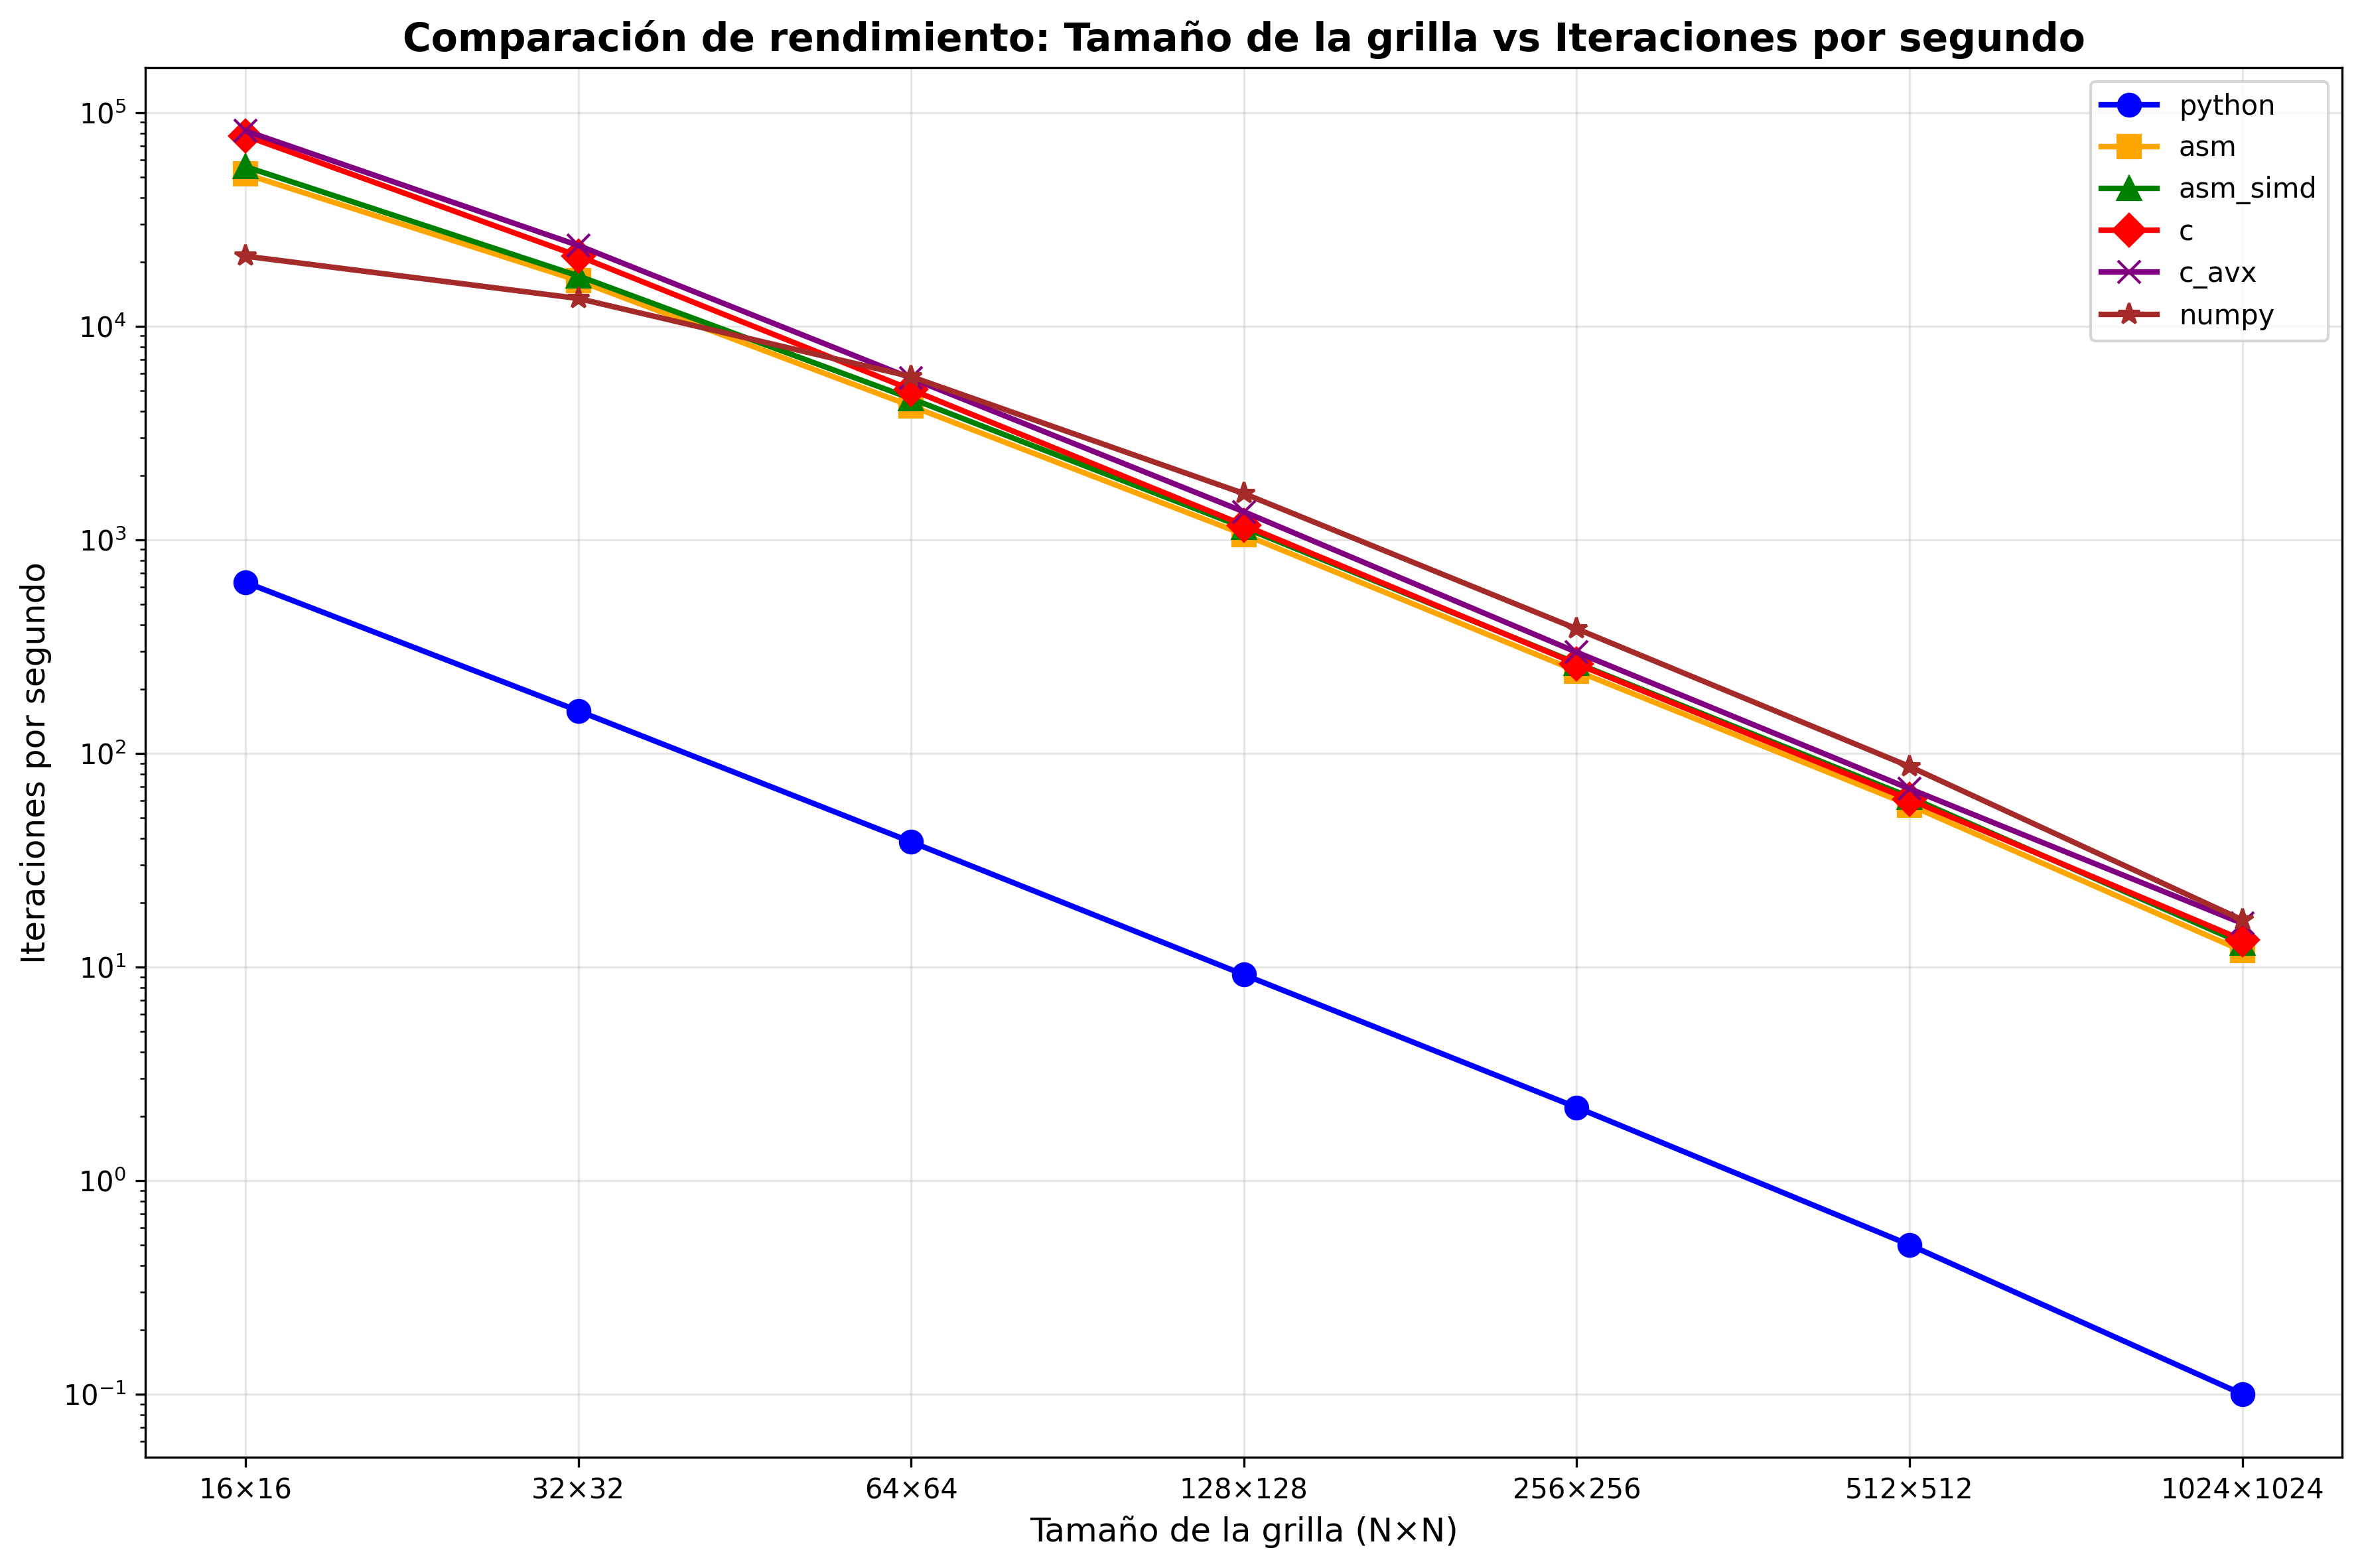
\includegraphics[width=\textwidth]{extra/steps_per_second.png}
        \caption{Comparación rendimiento entre los distintos backends. Se utiliza escala logaritmica en ambos ejes.}
        \label{fig:performance}
    \end{minipage}
    \hfill
    \begin{minipage}[t]{0.48\textwidth}
        \centering
        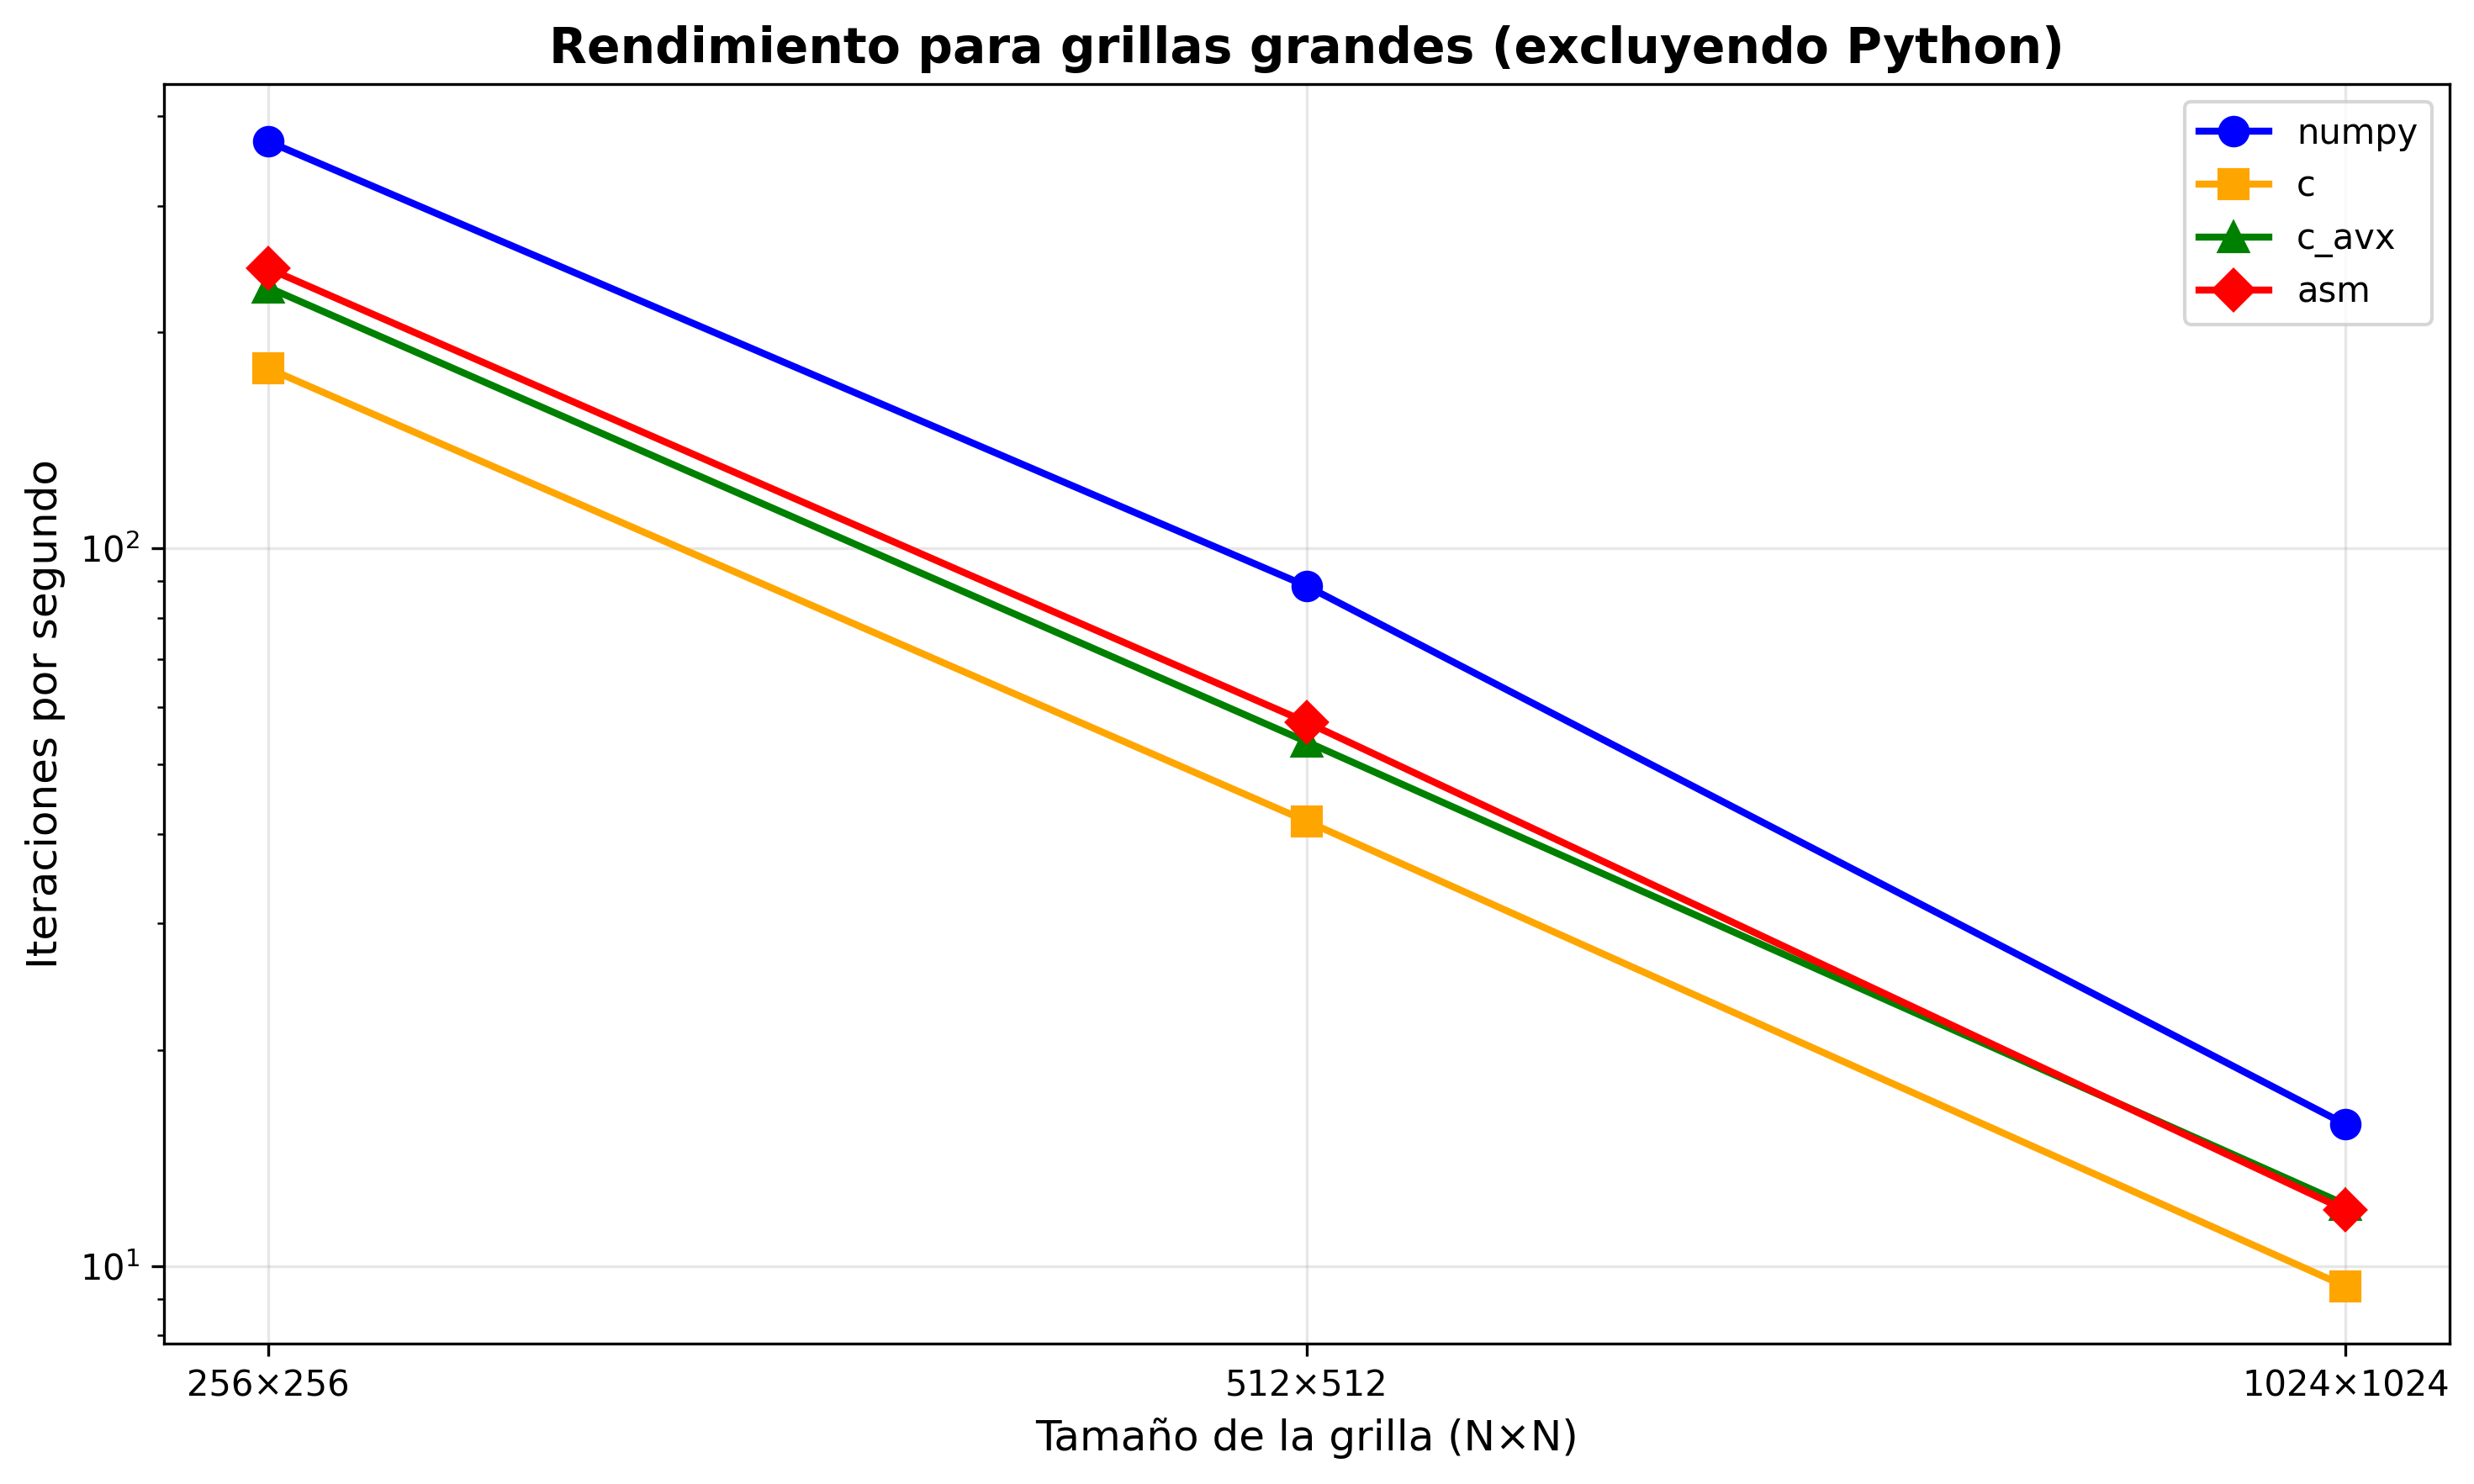
\includegraphics[width=\textwidth]{extra/steps_per_second_top3.png}
        \caption{Comparación detallada del rendimiento de las implementaciones rapidas en grillas grandes.}
        \label{fig:performance_top3}
    \end{minipage}
\end{figure}

\subsection{Analisis}

Los resultados experimentales presentados en \ref{tab:performance_results} revelan patrones interesantes en el rendimiento de las diferentes implementaciones:
\begin{itemize}
    \item \textbf{Python vs. Implementaciones Optimizadas:} La implementación en Python puro muestra un rendimiento dramáticamente inferior, siendo hasta 1000 veces más lenta que las implementaciones optimizadas.

    \item La implementacion en \textbf{C} es una alternativa excelente, combinando simplicidad de implementacion con buena performance. En los tamaños mas grandes, pierde con
          la version optimizada por AVX o la version acelerada con Assembler, pero se mantiene competitiva.

    \item \textbf{C + AVX} y \textbf{C + ASM} compiten por el segundo puesto, lo cual resulta interesante. Los dos metodos mejoran el rendimiento del backend en C pero implementan
          optimizaciones muy diferentes.

    \item \textbf{NumPy:} Domina consistentemente en grillas grandes, evidenciando la efectividad de bibliotecas altamente optimizadas.
\end{itemize}

\section{Conclusiones}

Este trabajo ha explorado la implementación y optimización de un simulador de ondas 2D basado en la Transformada de Fourier, evaluando diferentes enfoques de implementación desde Python puro hasta optimizaciones vectoriales con AVX. 

\printbibliography

\end{document}
